%!TeX spellcheck = fr-FR
\documentclass[thesis]{subfiles}

\begin{document}

\begin{otherlanguage}{french}

\renewcommand{\thesection}{\arabic{section}}
\renewcommand{\thesubsection}{\arabic{section}.\arabic{subsection}}
\renewcommand{\thefigure}{R\arabic{figure}}
\setcounter{figure}{0}
\titlecontents{section}[4.8em]{\addvspace{0.1em}}{\contentslabel{2.2em}}{}{\titlerule*[1pc]{.}\contentspage}[]

\chapter*{Résumé en français}
\startcontents[chapters]
\printpartialtoc

\section*{Introduction}

Les matériaux poreux sont des matériaux présentant une porosité structurelle
avec des cavités appelées \emph{pores} dans leur la structure tridimensionnelle.
Ce réseau de pores peuvent varier en homogénéité et en régularité, créant ainsi
une grande variété de matériaux poreux. Ils ont tous en commun une surface
spécifique, à savoir la surface interne accessible par grammes de matériau,
élevée --- jusqu'à des milliers de mètres carrés par gramme de
matériau\cite{Farha2012} dans les cas les plus extrêmes. Cette très grande
surface spécifique est exploitée dans nombre d'applications industrielles
importantes, notamment dans les domaines de l'adsorption et de la catalyse. Par
exemple, ils sont utilisés pour séparer dans des mélanges de gaz ou de liquide
sous forme de tamis moléculaires; pour filtrer et éliminer les métaux lourds
dans l'eau ou comme catalyseurs hétérogènes dans les raffineries pétrolières
lors du procédé de craquage.

L'union internationale de chimie pure et appliquée (IUPAC) recommande une
classification des matériaux poreux en trois groupes, selon la taille des
pores\cite{Rouquerol1994}. On trouve tout d'abord les solides
\emph{microporeux}, dont les pores ont un diamètre inférieur à \SI{2}{nm}. Les
solides \emph{mésoporeux} ont des pores dont le diamètre est compris entre 2 et
\SI{50}{nm}. Enfin, les solides avec pores plus grands que \SI{50}{nm} sont dit
\emph{macroporeux}. Les solides microporeux et mésoporeux sont souvent regroupés
sous l'appellation de solides \emph{nanoporeux}, dans lesquels la taille des
pores ne dépasse pas \SI{50}{nm}.

Deux familles de matériaux nanoporeux cristallins sont particulièrement
intéressantes. Tout d'abord, les zéolithes sont des aluminosilicates poreux
naturels et artificiels connus depuis 1756 et synthétisé artificiellement depuis
les années 1940. Elles sont actuellement très utilisées industriellement, en
particulier comme catalyseurs dans l'industrie pétrolière et comme adoucisseurs
d'eau dans les lessives. Depuis les années 2000, une nouvelle famille de
matériaux nanoporeux cristallins hybride organiques--inorganiques appelés
\emph{Metal--Organic Frameworks} (MOF) ont été découvert et ont suscité
l'intérêt de la communauté scientifique. Ces nouveaux matériaux sont construits
à partir de centres métalliques, reliées entre eux par des ligands organiques.
Cette méthode de construction permet un très grand éventail de structures
différentes, et ouvre la voie à des matériaux conçu pour une application
spécifique. En changeant la combinaison de ligands et métaux utilisés, il est
possible de changer la taille, la forme et le comportement physico-chimique des
pores, comme illustré sur la figure~\ref{fig:fr:mof-different-linkers}.

\begin{figure}[ht]
    \centering
    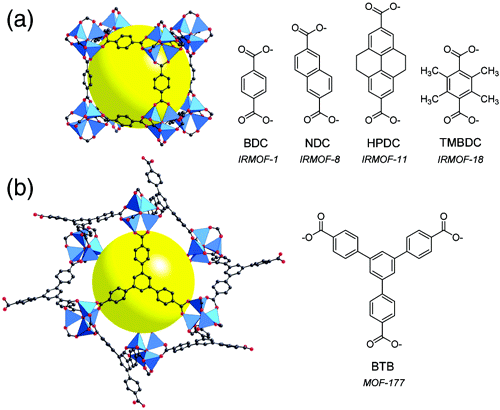
\includegraphics[width=0.65\textwidth]{figures/cited/mof-different-linker}
    \caption{Deux exemples de MOFs construit avec un centre métallique zinc.
    (a) Structure de la MOF-5, avec un ligand linéaire. (b) Structure de la
    MOF-177, avec un ligand trigonal. Reproduit avec permission de la
    référence~\cite{Rowsell2004}, copyright (2004) American Chemical Society.}
    \label{fig:fr:mof-different-linkers}
\end{figure}

La faiblesse relative des liaisons de coordination entre les cations métalliques
et les ligands organiques est à l'origine d'une flexibilité structurelle
intrinsèque dans les MOFs, qui peut être locale ou étendue à l'ensemble du
matériau. Certain MOF, regroupés sous l'appellation \emph{"soft porous
crystals"}, réagissent à des stimuli externes comme la température, la pression,
l'adsorption de gaz ou même l'exposition à la lumière avec des modifications de
grande envergure de leur structure. Les différents modes de flexibilité pouvant
exister dans les MOFs sont représentés en figure~\ref{fig:fr:mof-flexibility}.
Si tous les MOFs peuvent présenter des déformations locales comme la rotation de
ligands, seuls les \emph{soft porous crystals} présente des déformations
globale. Par exemple, les matériaux de la famille MIL-53 présentent pendant
l'adsorption de gaz deux transitions de phase, allant d'une phase à pores
ouverts à une phase à pores fermés, puis de nouveau à la phase à pores
ouverts\cite{Serre2002} lorsque l'on augmente de manière continue de la quantité
de gaz adsorbé, donnant l'impression d'une \emph{respiration} du matériau.

\begin{figure}[ht]
    \centering
    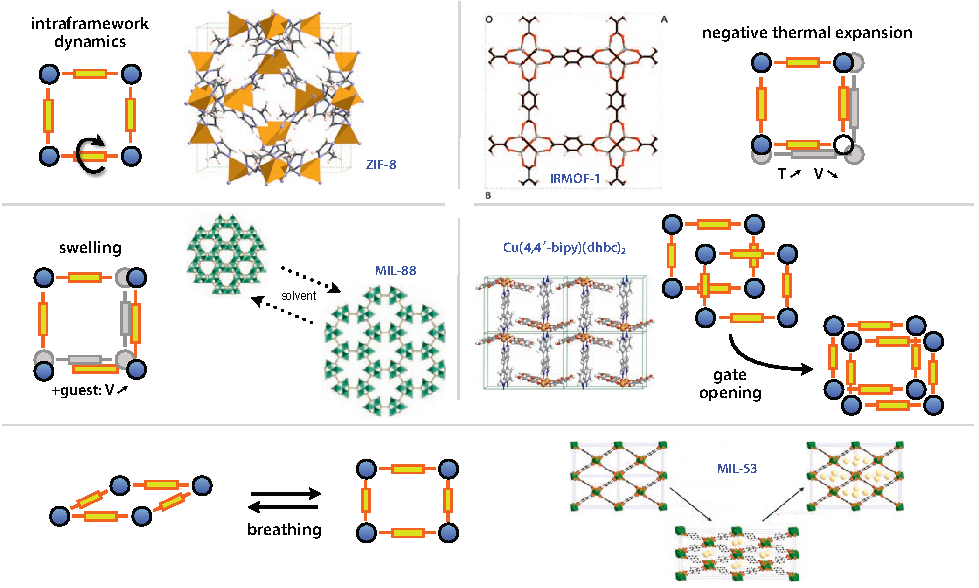
\includegraphics[width=\textwidth]{figures/cited/mof-flexibility}
    \caption{Illustration des principaux modes de flexibilité des MOFs: rotation
    de ligands, expansion thermique, gonflement, ouverture de porte et
    respiration. Reproduit avec permission de la référence~\cite{Coudert2011},
    copyright (2011) Wiley.}
    \label{fig:fr:mof-flexibility}
\end{figure}

La plupart des applications des matériaux nanoporeux sont liées à l'entrée
d'autres espèces chimiques (en phase liquide ou gazeuse) à l'intérieur des pores
du matériau. Lorsque le fluide à l'extérieur est dans l'état gazeux, le
processus est appelé adsorption, tandis que pour les liquides on parle
d'intrusion. L'adsorption et l'intrusion ont tous deux un effet sur les
propriétés physiques et chimiques du fluide confiné dans les nanopores. Les
fluides confinés sont généralement organisés plus régulièrement, prenant ainsi
l'aspect d'une phase solide tout en restant mobiles. L'inverse est également
vrai: la présence du fluide à l'intérieur des pores peut modifier les propriétés
et le comportement du matériau environnant. Les matériaux flexibles sont
particulièrement touchés et peuvent subir des transitions de phase induites par
l'adsorption, entraînant des phénomènes macroscopiques comme une
\emph{"ouverture de portes"} (\emph{gate-opening}), la respiration ou
l'adsorption négative de gaz. Le couplage entre l'adsorption ou l'intrusion et
les changements de structure des matériaux nanoporeux flexibles est difficile à
étudier, car il implique des équilibres de phases entre les fluides confinés et
à l'état pur, ainsi que l'équilibre entre différentes phases du matériau.

Pendant ma thèse, je me suis intéressé à la simulation moléculaire de
l'adsorption et de l'intrusion de fluides dans les matériaux nanoporeux
flexibles. Les outils de simulation moléculaire peuvent accélérer le
développement de nouveaux matériaux adaptés à des applications spécifiques. La
prédiction des propriétés de ces matériaux avant leur synthèse réduit fortement
le coût de création de nouveaux matériaux. Les propriétés qui peuvent être
étudiées et la fiabilité des prédictions correspondantes dépendent des
techniques utilisées pour modéliser les systèmes en question. Au cours de ma
thèse, j'ai utilisé plusieurs techniques à différentes échelles de temps et de
taille pour étudier l'adsorption et l'intrusion dans les matériaux poreux
flexibles, et leurs effets tant sur le fluide confiné que les matériaux. J'ai
ainsi utilisé des modèles basés sur la thermodynamique classique pour l'étude de
la co-adsorption des gaz, des simulations \emph{"umbrella sampling"} pour
extraire des profils d'énergie libre d'intrusion de l'eau, la dynamique
moléculaire classique et les simulations Monte-Carlo classiques pour l'intrusion
d'eau et de solutions aqueuses dans des matériaux rigides et flexibles, et des
simulations de dynamique moléculaire \abinitio pour étudier l'organisation
moléculaire des fluides dans des pores.

\clearpage
\section{Séparation de gaz dans des matériaux flexibles}

\begin{figure}[h]
    \centering
    \raisebox{-0.5\height}{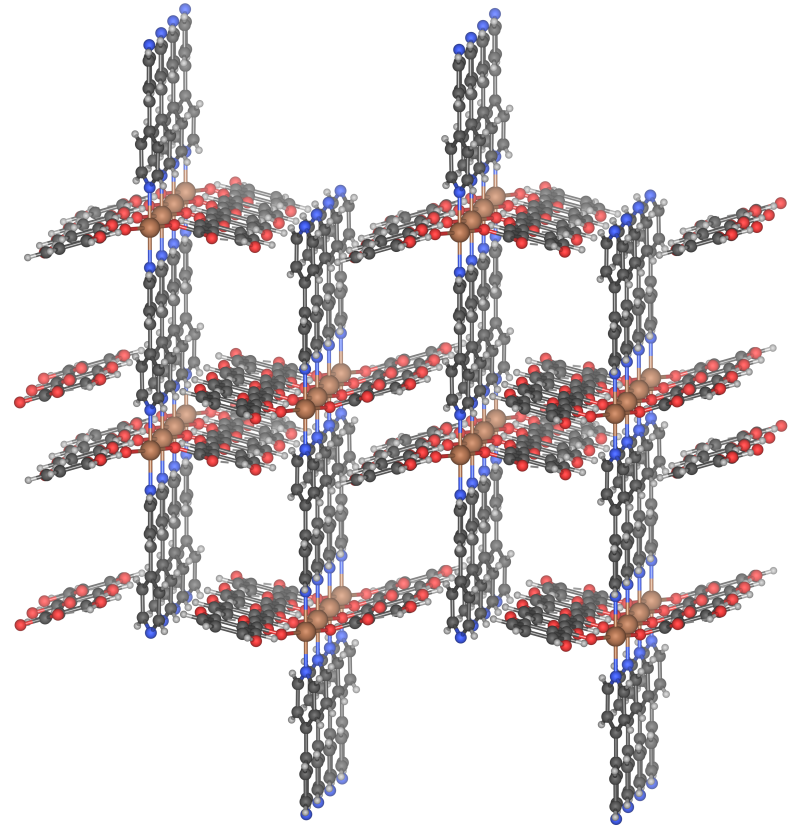
\includegraphics[width=0.32\textwidth]{figures/images/cu-dhbc-structure}}
    \hfill
    \raisebox{-0.5\height}{% GNUPLOT: LaTeX picture with Postscript
\begingroup
  \makeatletter
  \providecommand\color[2][]{%
    \GenericError{(gnuplot) \space\space\space\@spaces}{%
      Package color not loaded in conjunction with
      terminal option `colourtext'%
    }{See the gnuplot documentation for explanation.%
    }{Either use 'blacktext' in gnuplot or load the package
      color.sty in LaTeX.}%
    \renewcommand\color[2][]{}%
  }%
  \providecommand\includegraphics[2][]{%
    \GenericError{(gnuplot) \space\space\space\@spaces}{%
      Package graphicx or graphics not loaded%
    }{See the gnuplot documentation for explanation.%
    }{The gnuplot epslatex terminal needs graphicx.sty or graphics.sty.}%
    \renewcommand\includegraphics[2][]{}%
  }%
  \providecommand\rotatebox[2]{#2}%
  \@ifundefined{ifGPcolor}{%
    \newif\ifGPcolor
    \GPcolortrue
  }{}%
  \@ifundefined{ifGPblacktext}{%
    \newif\ifGPblacktext
    \GPblacktextfalse
  }{}%
  % define a \g@addto@macro without @ in the name:
  \let\gplgaddtomacro\g@addto@macro
  % define empty templates for all commands taking text:
  \gdef\gplbacktext{}%
  \gdef\gplfronttext{}%
  \makeatother
  \ifGPblacktext
    % no textcolor at all
    \def\colorrgb#1{}%
    \def\colorgray#1{}%
  \else
    % gray or color?
    \ifGPcolor
      \def\colorrgb#1{\color[rgb]{#1}}%
      \def\colorgray#1{\color[gray]{#1}}%
      \expandafter\def\csname LTw\endcsname{\color{white}}%
      \expandafter\def\csname LTb\endcsname{\color{black}}%
      \expandafter\def\csname LTa\endcsname{\color{black}}%
      \expandafter\def\csname LT0\endcsname{\color[rgb]{1,0,0}}%
      \expandafter\def\csname LT1\endcsname{\color[rgb]{0,1,0}}%
      \expandafter\def\csname LT2\endcsname{\color[rgb]{0,0,1}}%
      \expandafter\def\csname LT3\endcsname{\color[rgb]{1,0,1}}%
      \expandafter\def\csname LT4\endcsname{\color[rgb]{0,1,1}}%
      \expandafter\def\csname LT5\endcsname{\color[rgb]{1,1,0}}%
      \expandafter\def\csname LT6\endcsname{\color[rgb]{0,0,0}}%
      \expandafter\def\csname LT7\endcsname{\color[rgb]{1,0.3,0}}%
      \expandafter\def\csname LT8\endcsname{\color[rgb]{0.5,0.5,0.5}}%
    \else
      % gray
      \def\colorrgb#1{\color{black}}%
      \def\colorgray#1{\color[gray]{#1}}%
      \expandafter\def\csname LTw\endcsname{\color{white}}%
      \expandafter\def\csname LTb\endcsname{\color{black}}%
      \expandafter\def\csname LTa\endcsname{\color{black}}%
      \expandafter\def\csname LT0\endcsname{\color{black}}%
      \expandafter\def\csname LT1\endcsname{\color{black}}%
      \expandafter\def\csname LT2\endcsname{\color{black}}%
      \expandafter\def\csname LT3\endcsname{\color{black}}%
      \expandafter\def\csname LT4\endcsname{\color{black}}%
      \expandafter\def\csname LT5\endcsname{\color{black}}%
      \expandafter\def\csname LT6\endcsname{\color{black}}%
      \expandafter\def\csname LT7\endcsname{\color{black}}%
      \expandafter\def\csname LT8\endcsname{\color{black}}%
    \fi
  \fi
    \setlength{\unitlength}{0.0500bp}%
    \ifx\gptboxheight\undefined%
      \newlength{\gptboxheight}%
      \newlength{\gptboxwidth}%
      \newsavebox{\gptboxtext}%
    \fi%
    \setlength{\fboxrule}{0.5pt}%
    \setlength{\fboxsep}{1pt}%
\begin{picture}(4520.00,3400.00)%
    \gplgaddtomacro\gplbacktext{%
      \csname LTb\endcsname%%
      \put(441,595){\makebox(0,0)[r]{\strut{}$0$}}%
      \csname LTb\endcsname%%
      \put(441,1468){\makebox(0,0)[r]{\strut{}$1$}}%
      \csname LTb\endcsname%%
      \put(441,2340){\makebox(0,0)[r]{\strut{}$2$}}%
      \csname LTb\endcsname%%
      \put(441,3213){\makebox(0,0)[r]{\strut{}$3$}}%
      \csname LTb\endcsname%%
      \put(543,409){\makebox(0,0){\strut{}$0$}}%
      \csname LTb\endcsname%%
      \put(1461,409){\makebox(0,0){\strut{}$20$}}%
      \csname LTb\endcsname%%
      \put(2378,409){\makebox(0,0){\strut{}$40$}}%
      \csname LTb\endcsname%%
      \put(3296,409){\makebox(0,0){\strut{}$60$}}%
      \csname LTb\endcsname%%
      \put(4213,409){\makebox(0,0){\strut{}$80$}}%
    }%
    \gplgaddtomacro\gplfronttext{%
      \csname LTb\endcsname%%
      \put(153,1904){\rotatebox{-270}{\makebox(0,0){\strut{}uptake / (mol/mol)}}}%
      \csname LTb\endcsname%%
      \put(2378,130){\makebox(0,0){\strut{}pressure / atm}}%
      \csname LTb\endcsname%%
      \put(3425,1271){\makebox(0,0)[r]{\strut{}CH$_4$}}%
      \csname LTb\endcsname%%
      \put(3425,1030){\makebox(0,0)[r]{\strut{}CO$_2$}}%
      \csname LTb\endcsname%%
      \put(3425,789){\makebox(0,0)[r]{\strut{}O$_2$}}%
    }%
    \gplbacktext
    \put(0,0){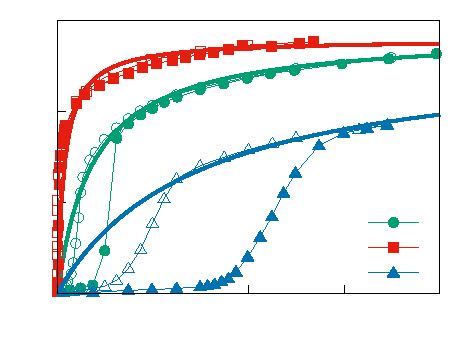
\includegraphics{cu-dhbc}}%
    \gplfronttext
  \end{picture}%
\endgroup
}
    \vskip-1em
    \caption{(gauche) Structure de \Cudhbc. (droite) Isothermes d'adsorption à
    \SI{298}{K} dans \Cudhbc pour différents gaz. L'adsorption est représenté
    en symboles plein, la desorption en symboles creux. Les données
    expérimentale ont été publiées par \citeauthor{Kitaura2003}\cite{Kitaura2003}}
    \label{fig:fr:cu-dhbc}
\end{figure}

La séparation de gaz est une étape importante dans de multiples procédés
industriels, allant de séparation des hydrocarbures dans la chimie du pétrole, à
la séparation et stockage du \ce{CO2} ou l'extraction d'oxygène dans l'air. Les
deux principales méthodes utilisées pour la séparation des gaz sont la
distillation cryogénique, principalement utilisée pour la séparation de l'air,
et l'adsorption différentielle. Les procédés de séparation des gaz basés sur
l'adsorption sont très polyvalents grâce au large choix de matériaux
disponibles, et de la possibilité d'adapter l'adsorbant à un système de gaz
spécifique. Le choix d'un adsorbant et la taille d'une unité de production de
séparation d'un mélange gazeux, nécessite une bonne connaissance des propriétés
de co-adsorption de ces gaz.

La caractérisation expérimentale de la co-adsorption est en général longue et
couteuse, à cause du grand nombre de paramètres à faire varier. Ce coût
important est à l'origine de plusieurs modèles théoriques permettant de prédire
la co-adsorption à partir de données d'adsorption de corps purs. La méthode la
plus couramment utilisée sur la théorie des solutions adsorbée idéale
(\emph{Ideal Adsorbed Solution Theory}, IAST)\cite{Myers1965}, qui est robuste
et relativement simple à mettre en œuvre. En pratique, l'utilisation de la
méthode IAST revient à travailler dans l'ensemble thermodynamique
grand-canonique, et à considérer la matrice d'adsorption comme étant rigide.
Pour pouvoir décrire la flexibilité des matériaux lors de l'adsorption, il faut
utiliser l'ensemble osmotique à la place. Cet ensemble est à la base de la
méthode OFAST (\emph{Osmotic Framework Adsorbed Solution Theory}) développée
dans le groupe\cite{Coudert2010, Ortiz2011}. Pour une description plus en détail
de ces méthodes, je renvoie le lecteur au chapitre~\ref{sec:macroscopic} de ce
manuscrit ou à l'article correspondant\cite{Fraux2018}.

Durant ma thèse, j'ai utilisé à la fois IAST et OFAST pour calculer la
sélectivité d'adsorption dans les MOFs \Cudhbc et \RPMZn, et démontrer
l'inadéquation d'IAST lorsque les structures adsorbantes sont flexibles. Je
vais rappeler rapidement ici les résultats obtenus dans le cas de \Cudhbc.
L'adsorption dans ce matériau, présenté en figure~\ref{fig:fr:cu-dhbc}, est
représentatif du phénomène d'ouverture de portes: en dessus d'une pression
"d'ouverture", aucune molécule de gaz n'entre dans la structure, et au-delà de
cette pression l'adsorption se produit normalement. La sélectivité prédite à
partir de ces isothermes d'adsorption par IAST et OFAST est présentée en
figure~\ref{fig:fr:cu-dhbc:iast-ofast:selectivity}.

\begin{figure}[t]
    \centering
    % GNUPLOT: LaTeX picture with Postscript
\begingroup
  \makeatletter
  \providecommand\color[2][]{%
    \GenericError{(gnuplot) \space\space\space\@spaces}{%
      Package color not loaded in conjunction with
      terminal option `colourtext'%
    }{See the gnuplot documentation for explanation.%
    }{Either use 'blacktext' in gnuplot or load the package
      color.sty in LaTeX.}%
    \renewcommand\color[2][]{}%
  }%
  \providecommand\includegraphics[2][]{%
    \GenericError{(gnuplot) \space\space\space\@spaces}{%
      Package graphicx or graphics not loaded%
    }{See the gnuplot documentation for explanation.%
    }{The gnuplot epslatex terminal needs graphicx.sty or graphics.sty.}%
    \renewcommand\includegraphics[2][]{}%
  }%
  \providecommand\rotatebox[2]{#2}%
  \@ifundefined{ifGPcolor}{%
    \newif\ifGPcolor
    \GPcolortrue
  }{}%
  \@ifundefined{ifGPblacktext}{%
    \newif\ifGPblacktext
    \GPblacktextfalse
  }{}%
  % define a \g@addto@macro without @ in the name:
  \let\gplgaddtomacro\g@addto@macro
  % define empty templates for all commands taking text:
  \gdef\gplbacktext{}%
  \gdef\gplfronttext{}%
  \makeatother
  \ifGPblacktext
    % no textcolor at all
    \def\colorrgb#1{}%
    \def\colorgray#1{}%
  \else
    % gray or color?
    \ifGPcolor
      \def\colorrgb#1{\color[rgb]{#1}}%
      \def\colorgray#1{\color[gray]{#1}}%
      \expandafter\def\csname LTw\endcsname{\color{white}}%
      \expandafter\def\csname LTb\endcsname{\color{black}}%
      \expandafter\def\csname LTa\endcsname{\color{black}}%
      \expandafter\def\csname LT0\endcsname{\color[rgb]{1,0,0}}%
      \expandafter\def\csname LT1\endcsname{\color[rgb]{0,1,0}}%
      \expandafter\def\csname LT2\endcsname{\color[rgb]{0,0,1}}%
      \expandafter\def\csname LT3\endcsname{\color[rgb]{1,0,1}}%
      \expandafter\def\csname LT4\endcsname{\color[rgb]{0,1,1}}%
      \expandafter\def\csname LT5\endcsname{\color[rgb]{1,1,0}}%
      \expandafter\def\csname LT6\endcsname{\color[rgb]{0,0,0}}%
      \expandafter\def\csname LT7\endcsname{\color[rgb]{1,0.3,0}}%
      \expandafter\def\csname LT8\endcsname{\color[rgb]{0.5,0.5,0.5}}%
    \else
      % gray
      \def\colorrgb#1{\color{black}}%
      \def\colorgray#1{\color[gray]{#1}}%
      \expandafter\def\csname LTw\endcsname{\color{white}}%
      \expandafter\def\csname LTb\endcsname{\color{black}}%
      \expandafter\def\csname LTa\endcsname{\color{black}}%
      \expandafter\def\csname LT0\endcsname{\color{black}}%
      \expandafter\def\csname LT1\endcsname{\color{black}}%
      \expandafter\def\csname LT2\endcsname{\color{black}}%
      \expandafter\def\csname LT3\endcsname{\color{black}}%
      \expandafter\def\csname LT4\endcsname{\color{black}}%
      \expandafter\def\csname LT5\endcsname{\color{black}}%
      \expandafter\def\csname LT6\endcsname{\color{black}}%
      \expandafter\def\csname LT7\endcsname{\color{black}}%
      \expandafter\def\csname LT8\endcsname{\color{black}}%
    \fi
  \fi
    \setlength{\unitlength}{0.0500bp}%
    \ifx\gptboxheight\undefined%
      \newlength{\gptboxheight}%
      \newlength{\gptboxwidth}%
      \newsavebox{\gptboxtext}%
    \fi%
    \setlength{\fboxrule}{0.5pt}%
    \setlength{\fboxsep}{1pt}%
\begin{picture}(7360.00,6800.00)%
    \gplgaddtomacro\gplbacktext{%
      \csname LTb\endcsname%%
      \put(747,4971){\makebox(0,0)[r]{\strut{}$0$}}%
      \csname LTb\endcsname%%
      \put(747,5628){\makebox(0,0)[r]{\strut{}$1000$}}%
      \csname LTb\endcsname%%
      \put(747,6285){\makebox(0,0)[r]{\strut{}$2000$}}%
      \csname LTb\endcsname%%
      \put(849,4719){\makebox(0,0){\strut{}$0$}}%
      \csname LTb\endcsname%%
      \put(1480,4719){\makebox(0,0){\strut{}$20$}}%
      \csname LTb\endcsname%%
      \put(2111,4719){\makebox(0,0){\strut{}$40$}}%
      \csname LTb\endcsname%%
      \put(2742,4719){\makebox(0,0){\strut{}$60$}}%
      \csname LTb\endcsname%%
      \put(3373,4719){\makebox(0,0){\strut{}$80$}}%
    }%
    \gplgaddtomacro\gplfronttext{%
      \csname LTb\endcsname%%
      \put(153,5759){\rotatebox{-270}{\makebox(0,0){\strut{}\ce{CO2} / \ce{O2} selectivity}}}%
      \csname LTb\endcsname%%
      \put(2585,6418){\makebox(0,0)[r]{\strut{}$y_{\ce{CO2}} = 0.1$}}%
      \csname LTb\endcsname%%
      \put(2585,6177){\makebox(0,0)[r]{\strut{}$y_{\ce{CO2}} = 0.5$}}%
      \csname LTb\endcsname%%
      \put(2585,5936){\makebox(0,0)[r]{\strut{}$y_{\ce{CO2}} = 0.9$}}%
    }%
    \gplgaddtomacro\gplbacktext{%
      \csname LTb\endcsname%%
      \put(4241,4905){\makebox(0,0)[r]{\strut{}$1$}}%
      \csname LTb\endcsname%%
      \put(4241,5343){\makebox(0,0)[r]{\strut{}$10$}}%
      \csname LTb\endcsname%%
      \put(4241,5780){\makebox(0,0)[r]{\strut{}$100$}}%
      \csname LTb\endcsname%%
      \put(4241,6218){\makebox(0,0)[r]{\strut{}$1000$}}%
      \csname LTb\endcsname%%
      \put(4343,4719){\makebox(0,0){\strut{}$0$}}%
      \csname LTb\endcsname%%
      \put(5021,4719){\makebox(0,0){\strut{}$20$}}%
      \csname LTb\endcsname%%
      \put(5698,4719){\makebox(0,0){\strut{}$40$}}%
      \csname LTb\endcsname%%
      \put(6376,4719){\makebox(0,0){\strut{}$60$}}%
      \csname LTb\endcsname%%
      \put(7053,4719){\makebox(0,0){\strut{}$80$}}%
    }%
    \gplgaddtomacro\gplfronttext{%
    }%
    \gplgaddtomacro\gplbacktext{%
      \csname LTb\endcsname%%
      \put(543,2719){\makebox(0,0)[r]{\strut{}$0$}}%
      \csname LTb\endcsname%%
      \put(543,3533){\makebox(0,0)[r]{\strut{}$5$}}%
      \csname LTb\endcsname%%
      \put(543,4347){\makebox(0,0)[r]{\strut{}$10$}}%
      \csname LTb\endcsname%%
      \put(645,2452){\makebox(0,0){\strut{}$0$}}%
      \csname LTb\endcsname%%
      \put(1327,2452){\makebox(0,0){\strut{}$20$}}%
      \csname LTb\endcsname%%
      \put(2009,2452){\makebox(0,0){\strut{}$40$}}%
      \csname LTb\endcsname%%
      \put(2691,2452){\makebox(0,0){\strut{}$60$}}%
      \csname LTb\endcsname%%
      \put(3373,2452){\makebox(0,0){\strut{}$80$}}%
    }%
    \gplgaddtomacro\gplfronttext{%
      \csname LTb\endcsname%%
      \put(153,3492){\rotatebox{-270}{\makebox(0,0){\strut{}\ce{CH4} / \ce{O2} selectivity}}}%
    }%
    \gplgaddtomacro\gplbacktext{%
      \csname LTb\endcsname%%
      \put(4037,2638){\makebox(0,0)[r]{\strut{}$1$}}%
      \csname LTb\endcsname%%
      \put(4037,4347){\makebox(0,0)[r]{\strut{}$10$}}%
      \csname LTb\endcsname%%
      \put(4139,2452){\makebox(0,0){\strut{}$0$}}%
      \csname LTb\endcsname%%
      \put(4868,2452){\makebox(0,0){\strut{}$20$}}%
      \csname LTb\endcsname%%
      \put(5596,2452){\makebox(0,0){\strut{}$40$}}%
      \csname LTb\endcsname%%
      \put(6325,2452){\makebox(0,0){\strut{}$60$}}%
      \csname LTb\endcsname%%
      \put(7053,2452){\makebox(0,0){\strut{}$80$}}%
    }%
    \gplgaddtomacro\gplfronttext{%
    }%
    \gplgaddtomacro\gplbacktext{%
      \csname LTb\endcsname%%
      \put(645,595){\makebox(0,0)[r]{\strut{}$0$}}%
      \csname LTb\endcsname%%
      \put(645,1338){\makebox(0,0)[r]{\strut{}$0.5$}}%
      \csname LTb\endcsname%%
      \put(645,2080){\makebox(0,0)[r]{\strut{}$1$}}%
      \csname LTb\endcsname%%
      \put(747,409){\makebox(0,0){\strut{}$0$}}%
      \csname LTb\endcsname%%
      \put(1404,409){\makebox(0,0){\strut{}$20$}}%
      \csname LTb\endcsname%%
      \put(2060,409){\makebox(0,0){\strut{}$40$}}%
      \csname LTb\endcsname%%
      \put(2717,409){\makebox(0,0){\strut{}$60$}}%
      \csname LTb\endcsname%%
      \put(3373,409){\makebox(0,0){\strut{}$80$}}%
    }%
    \gplgaddtomacro\gplfronttext{%
      \csname LTb\endcsname%%
      \put(153,1337){\rotatebox{-270}{\makebox(0,0){\strut{}\ce{CH4} / \ce{CO2} selectivity}}}%
      \csname LTb\endcsname%%
      \put(2060,130){\makebox(0,0){\strut{}pressure / atm}}%
    }%
    \gplgaddtomacro\gplbacktext{%
      \csname LTb\endcsname%%
      \put(4241,595){\makebox(0,0)[r]{\strut{}$0.01$}}%
      \csname LTb\endcsname%%
      \put(4241,1338){\makebox(0,0)[r]{\strut{}$0.1$}}%
      \csname LTb\endcsname%%
      \put(4241,2080){\makebox(0,0)[r]{\strut{}$1$}}%
      \csname LTb\endcsname%%
      \put(4343,409){\makebox(0,0){\strut{}$0$}}%
      \csname LTb\endcsname%%
      \put(5021,409){\makebox(0,0){\strut{}$20$}}%
      \csname LTb\endcsname%%
      \put(5698,409){\makebox(0,0){\strut{}$40$}}%
      \csname LTb\endcsname%%
      \put(6376,409){\makebox(0,0){\strut{}$60$}}%
      \csname LTb\endcsname%%
      \put(7053,409){\makebox(0,0){\strut{}$80$}}%
    }%
    \gplgaddtomacro\gplfronttext{%
      \csname LTb\endcsname%%
      \put(5698,130){\makebox(0,0){\strut{}pressure / atm}}%
    }%
    \gplbacktext
    \put(0,0){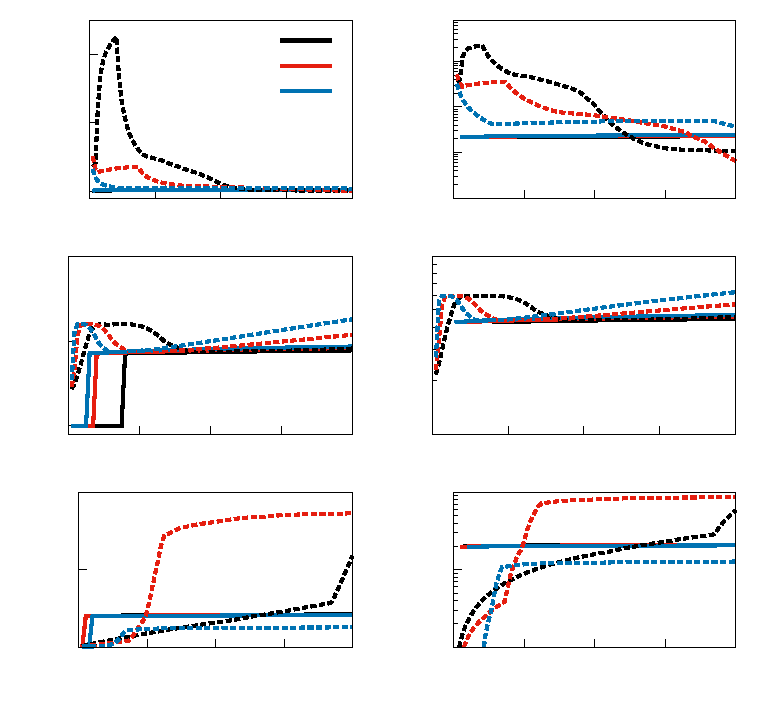
\includegraphics{cu-dhbc-selectivities}}%
    \gplfronttext
  \end{picture}%
\endgroup

    \vskip-3em
    \caption{Comparaison de la sélectivité prédite par la méthodes IAST (lignes
    pointillées) ou OFAST (lignes pleines) pour les couples \ce{CO2}/\ce{O2}
    (haut); \ce{CH4}/\ce{O2} (milieu) et \ce{CH4}/\ce{CO2} (bas) dans \Cudhbc;
    en échelle linéaire (gauche) et logarithmique (droite).}
    \vskip-1ex
    \label{fig:fr:cu-dhbc:iast-ofast:selectivity}
\end{figure}

La sélectivité d'adsorption calculée avec OFAST se comporte comme attendu: à
basse pression, les pores sont fermés et aucun gaz n'entre dans la structure.
Ensuite, à une pression dépendant de la composition de la phase gazeuse,
l'ouverture de porte se produit. Pour les pressions plus importantes, le
matériau est sous sa forme ouverte, et la valeur de sélectivité dépend de la
différence en capacité d'absorption entre les deux gaz, environ 20 pour les
mélanges \ce{CO2}/\ce{O2} et 4 pour les mélanges \ce{CH4}/\ce{O2}. Au contraire,
les sélectivités calculées par la méthode IAST sont clairement non physiques.
Toutes les courbes de sélectivité présentent un maximum dans la plage de
pression où se produit l'ouverture de la structure, avec des sélectivités qui
peuvent être plusieurs ordres de grandeur trop élevées, par exemple 2 000 au
lieu de 20 pour \ce{CO2}/\ce{O2}. Même loin de la pression de transition, les
sélectivités prédites par IAST ne reproduisent pas celles calculées avec OFAST,
le comportement incorrect à basse pression affectant directement les calculs
au-delà. J'ai donc pu confirmer par une étude quantitative que IAST n'est pas
adapté à l'adsorption dans les matériaux flexibles nanoporeux.

\clearpage
\section{Adsorption de \ce{N2} dans la \ZIF8}

Les ZIFs (\emph{zeolitic Imidazolate Frameworks}) sont une famille de MOFs
construits autour de centres métalliques tétravalents (Fe, Co, Zn, Cd, Cu)
assemblés par des ligands imidazolate ou imidazolate fonctionnalisés. Les
premières ZIF (ZIF-1 à ZIF-12) ont été synthétisés en 2006\cite{Park2006}, et se
sont révélés être plus résistantes à l'eau et la chaleur que les MOFs typiques,
ce qui les rend particulièrement attractif pour des applications commerciales.
J'ai spécifiquement étudié la \ZIF8 pendant ma thèse. Cette structure est
construite avec des ligands 2-méthyl-imidazolate (mim) et des ions \ce{Zn^2+}
comme centre métallique, assemblées dans une structure sodalite représentée en
figure~\ref{fig:zif8-ch3:structure}. Dans cette topologie, les pores principaux
sont quasi-sphériques et correspondent aux cages sodalite, reliés par des
fenêtres formées par 6 et 4 atomes de zinc. Deux nouveaux matériaux analogues à
\ZIF8 ont été synthétisés récemment par \citeauthor{Li2009}\cite{Li2009}
utilisant des ligands imidazolate chloro- et bromo-substitués à la place du
méthyl-imidazolate de la \ZIF8. Ces nouveaux matériaux, que nous appellerons
\ZIFCl et \ZIFBr, sont représentés dans la figure~\ref{fig:zif8x:structures}.

Les isothermes d'adsorption de l'azote à \SI{77}{K} dans \ZIF8, \ZIFCl et
\ZIFBr, sont présentés dans la figure~\ref{fig:zif8x:isotherms}. Elles ont été
mesurées dans le cadre d'une collaboration avec l'équipe expérimentale du
laboratoire IS2M de l'Université de Haute Alsace. Sur ces isothermes, nous
remarquons tout d'abord les deux sauts pour le cas de \ZIFCH3: un premier
correspondant au remplissage initial des pores jusqu'aux environs de
\SI{300}{cm^3/cm^3}, et un second jusqu'à \SI{400}{cm^3/cm^3}. Ce comportement
est celui d'une isotherme de type IV en la classification de
l'IUPAC\cite{Sing1985} (voir la figure~\ref{fig:iupac-isotherms}). Concernant
les deux nouveaux matériaux, l'adsorption dans la \ZIFCl se fait de la même
manière, avec une isotherme de type IV; alors que dans \ZIFBr, l'adsorption a
lieu avec une isotherme de type I, sans second saut dans la quantité adsorbée.
La présence du second saut dans les isothermes pour \ZIFCH3 et \ZIFCl est
surprenant ici, ce type d'isotherme étant en général associée à la présence de
plusieurs niveaux de porosités ou à des transitions de phase de l'hôte. Il
semblerait ici que la \ZIF8 subisse une transition de phase associée à une
rotation des ligands\cite{Moggach2009, FairenJimenez2011}.

Afin de mieux comprendre la relation entre la structure des ZIFs utilisées
l'adsorption de \ce{N2} dans ces ZIFs, j'ai utilisé des simulations de dynamique
moléculaire. Afin de pouvoir décrire pleinement la flexibilité de la \ZIF8, j'ai
favorisé la dynamique moléculaire \abinitio à la dynamique moléculaire
classique, basée sur un champ de force. Cette étude est publiée dans
\citejournal{Chaplais2018}\cite{Chaplais2018}.

\begin{figure}[ht]
    \centering
    % GNUPLOT: LaTeX picture with Postscript
\begingroup
  \makeatletter
  \providecommand\color[2][]{%
    \GenericError{(gnuplot) \space\space\space\@spaces}{%
      Package color not loaded in conjunction with
      terminal option `colourtext'%
    }{See the gnuplot documentation for explanation.%
    }{Either use 'blacktext' in gnuplot or load the package
      color.sty in LaTeX.}%
    \renewcommand\color[2][]{}%
  }%
  \providecommand\includegraphics[2][]{%
    \GenericError{(gnuplot) \space\space\space\@spaces}{%
      Package graphicx or graphics not loaded%
    }{See the gnuplot documentation for explanation.%
    }{The gnuplot epslatex terminal needs graphicx.sty or graphics.sty.}%
    \renewcommand\includegraphics[2][]{}%
  }%
  \providecommand\rotatebox[2]{#2}%
  \@ifundefined{ifGPcolor}{%
    \newif\ifGPcolor
    \GPcolortrue
  }{}%
  \@ifundefined{ifGPblacktext}{%
    \newif\ifGPblacktext
    \GPblacktextfalse
  }{}%
  % define a \g@addto@macro without @ in the name:
  \let\gplgaddtomacro\g@addto@macro
  % define empty templates for all commands taking text:
  \gdef\gplbacktext{}%
  \gdef\gplfronttext{}%
  \makeatother
  \ifGPblacktext
    % no textcolor at all
    \def\colorrgb#1{}%
    \def\colorgray#1{}%
  \else
    % gray or color?
    \ifGPcolor
      \def\colorrgb#1{\color[rgb]{#1}}%
      \def\colorgray#1{\color[gray]{#1}}%
      \expandafter\def\csname LTw\endcsname{\color{white}}%
      \expandafter\def\csname LTb\endcsname{\color{black}}%
      \expandafter\def\csname LTa\endcsname{\color{black}}%
      \expandafter\def\csname LT0\endcsname{\color[rgb]{1,0,0}}%
      \expandafter\def\csname LT1\endcsname{\color[rgb]{0,1,0}}%
      \expandafter\def\csname LT2\endcsname{\color[rgb]{0,0,1}}%
      \expandafter\def\csname LT3\endcsname{\color[rgb]{1,0,1}}%
      \expandafter\def\csname LT4\endcsname{\color[rgb]{0,1,1}}%
      \expandafter\def\csname LT5\endcsname{\color[rgb]{1,1,0}}%
      \expandafter\def\csname LT6\endcsname{\color[rgb]{0,0,0}}%
      \expandafter\def\csname LT7\endcsname{\color[rgb]{1,0.3,0}}%
      \expandafter\def\csname LT8\endcsname{\color[rgb]{0.5,0.5,0.5}}%
    \else
      % gray
      \def\colorrgb#1{\color{black}}%
      \def\colorgray#1{\color[gray]{#1}}%
      \expandafter\def\csname LTw\endcsname{\color{white}}%
      \expandafter\def\csname LTb\endcsname{\color{black}}%
      \expandafter\def\csname LTa\endcsname{\color{black}}%
      \expandafter\def\csname LT0\endcsname{\color{black}}%
      \expandafter\def\csname LT1\endcsname{\color{black}}%
      \expandafter\def\csname LT2\endcsname{\color{black}}%
      \expandafter\def\csname LT3\endcsname{\color{black}}%
      \expandafter\def\csname LT4\endcsname{\color{black}}%
      \expandafter\def\csname LT5\endcsname{\color{black}}%
      \expandafter\def\csname LT6\endcsname{\color{black}}%
      \expandafter\def\csname LT7\endcsname{\color{black}}%
      \expandafter\def\csname LT8\endcsname{\color{black}}%
    \fi
  \fi
    \setlength{\unitlength}{0.0500bp}%
    \ifx\gptboxheight\undefined%
      \newlength{\gptboxheight}%
      \newlength{\gptboxwidth}%
      \newsavebox{\gptboxtext}%
    \fi%
    \setlength{\fboxrule}{0.5pt}%
    \setlength{\fboxsep}{1pt}%
\begin{picture}(7760.00,3100.00)%
    \gplgaddtomacro\gplbacktext{%
      \csname LTb\endcsname%%
      \put(212,341){\makebox(0,0){\strut{}$0$}}%
      \csname LTb\endcsname%%
      \put(636,341){\makebox(0,0){\strut{}$10$}}%
      \csname LTb\endcsname%%
      \put(1060,341){\makebox(0,0){\strut{}$20$}}%
      \csname LTb\endcsname%%
      \put(1483,341){\makebox(0,0){\strut{}$30$}}%
      \csname LTb\endcsname%%
      \put(1907,341){\makebox(0,0){\strut{}$40$}}%
      \csname LTb\endcsname%%
      \put(2331,341){\makebox(0,0){\strut{}$50$}}%
    }%
    \gplgaddtomacro\gplfronttext{%
      \csname LTb\endcsname%%
      \put(1271,109){\makebox(0,0){\strut{}$\phi$ (°)}}%
      \csname LTb\endcsname%%
      \put(1271,2867){\makebox(0,0){\strut{}\ZIFCH3}}%
      \csname LTb\endcsname%%
      \put(1759,2494){\makebox(0,0)[r]{\strut{}\scriptsize 0 \ce{N2}}}%
      \csname LTb\endcsname%%
      \put(1759,2339){\makebox(0,0)[r]{\strut{}\scriptsize 10 \ce{N2}}}%
      \csname LTb\endcsname%%
      \put(1759,2184){\makebox(0,0)[r]{\strut{}\scriptsize 25 \ce{N2}}}%
      \csname LTb\endcsname%%
      \put(1759,2029){\makebox(0,0)[r]{\strut{}\scriptsize 40 \ce{N2}}}%
      \csname LTb\endcsname%%
      \put(1759,1874){\makebox(0,0)[r]{\strut{}\scriptsize 50 \ce{N2}}}%
    }%
    \gplgaddtomacro\gplbacktext{%
      \csname LTb\endcsname%%
      \put(2628,341){\makebox(0,0){\strut{}$0$}}%
      \csname LTb\endcsname%%
      \put(3086,341){\makebox(0,0){\strut{}$10$}}%
      \csname LTb\endcsname%%
      \put(3544,341){\makebox(0,0){\strut{}$20$}}%
      \csname LTb\endcsname%%
      \put(4001,341){\makebox(0,0){\strut{}$30$}}%
      \csname LTb\endcsname%%
      \put(4459,341){\makebox(0,0){\strut{}$40$}}%
      \csname LTb\endcsname%%
      \put(4917,341){\makebox(0,0){\strut{}$50$}}%
    }%
    \gplgaddtomacro\gplfronttext{%
      \csname LTb\endcsname%%
      \put(3772,109){\makebox(0,0){\strut{}$\phi$ (°)}}%
      \csname LTb\endcsname%%
      \put(3772,2867){\makebox(0,0){\strut{}\ZIFCl}}%
      \csname LTb\endcsname%%
      \put(4345,2494){\makebox(0,0)[r]{\strut{}\scriptsize 0 \ce{N2}}}%
      \csname LTb\endcsname%%
      \put(4345,2339){\makebox(0,0)[r]{\strut{}\scriptsize 10 \ce{N2}}}%
      \csname LTb\endcsname%%
      \put(4345,2184){\makebox(0,0)[r]{\strut{}\scriptsize 25 \ce{N2}}}%
      \csname LTb\endcsname%%
      \put(4345,2029){\makebox(0,0)[r]{\strut{}\scriptsize 40 \ce{N2}}}%
      \csname LTb\endcsname%%
      \put(4345,1874){\makebox(0,0)[r]{\strut{}\scriptsize 50 \ce{N2}}}%
    }%
    \gplgaddtomacro\gplbacktext{%
      \csname LTb\endcsname%%
      \put(5215,341){\makebox(0,0){\strut{}$0$}}%
      \csname LTb\endcsname%%
      \put(5673,341){\makebox(0,0){\strut{}$10$}}%
      \csname LTb\endcsname%%
      \put(6131,341){\makebox(0,0){\strut{}$20$}}%
      \csname LTb\endcsname%%
      \put(6588,341){\makebox(0,0){\strut{}$30$}}%
      \csname LTb\endcsname%%
      \put(7046,341){\makebox(0,0){\strut{}$40$}}%
      \csname LTb\endcsname%%
      \put(7504,341){\makebox(0,0){\strut{}$50$}}%
    }%
    \gplgaddtomacro\gplfronttext{%
      \csname LTb\endcsname%%
      \put(6359,109){\makebox(0,0){\strut{}$\phi$ (°)}}%
      \csname LTb\endcsname%%
      \put(6359,2867){\makebox(0,0){\strut{}\ZIFBr}}%
      \csname LTb\endcsname%%
      \put(6932,2494){\makebox(0,0)[r]{\strut{}\scriptsize 0 \ce{N2}}}%
      \csname LTb\endcsname%%
      \put(6932,2339){\makebox(0,0)[r]{\strut{}\scriptsize 8 \ce{N2}}}%
      \csname LTb\endcsname%%
      \put(6932,2184){\makebox(0,0)[r]{\strut{}\scriptsize 20 \ce{N2}}}%
      \csname LTb\endcsname%%
      \put(6932,2029){\makebox(0,0)[r]{\strut{}\scriptsize 40 \ce{N2}}}%
      \csname LTb\endcsname%%
      \put(6932,1874){\makebox(0,0)[r]{\strut{}\scriptsize 50 \ce{N2}}}%
    }%
    \gplbacktext
    \put(0,0){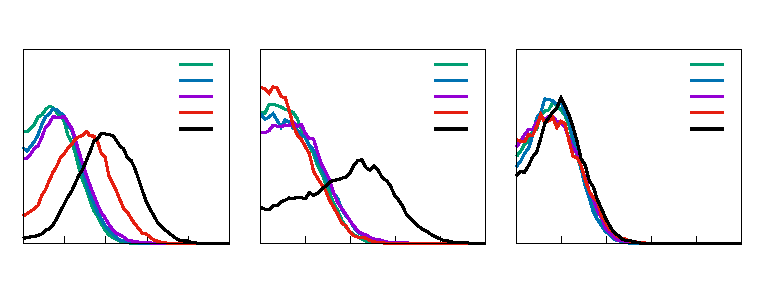
\includegraphics{zif8x-dihedrals}}%
    \gplfronttext
  \end{picture}%
\endgroup

    \caption{Distribution des angles dihèdre \ce{Zn-Zn-Zn-X} --- où \ce{X} est
    \ce{CH3}, \ce{Cl} or \ce{Br} selon la ZIF utilisée --- à différent
    remplissage d'azote.}
    \label{fig:fr:zif8x:dihedrals}
\end{figure}

Un premier indicateur de déformation de la structure est l'angle dièdre
\ce{Zn-Zn-Zn-Zn-Zn-X} --- présenté dans la figure~\ref{fig:zif8-ch3:structure}
--- où \ce{X} est \ce{CH3}, \ce{Cl} or \ce{Br} selon la ZIF utilisée. Il
représente la rotation des ligands autour du plan de la fenêtre à 6 éléments, 0°
étant le point où les ligands sont alignés avec ce plan. L'évolution de la
distribution de cet angle quand le remplissage augmente est représentée sur la
figure~\ref{fig:fr:zif8x:dihedrals}, où nous observons pour \ZIFCH3 une
augmentation progressive de la valeur moyenne de l'angle à mesure que la
quantité adsorbée augmente alors que la distribution reste gaussienne. Les deux
autres structures se comportent différemment. Pour \ZIFCl, presque aucun
changement n'est présent dans la distribution lors de l'adsorption jusqu'au
remplissage le plus élevé (\ie, $N = 50$). À ce moment, la distribution se
déplace et le profil n'est plus de type gaussien, mais ressemble à la somme de
deux distributions gaussiennes, l'une centrée autour de 25° et l'autre autour de
10°. Ceci indique vraisemblablement que certains des ligands ne tournent pas
même à fort remplissage. Enfin, pour \ZIFBr, aucun changement significatif ne se
produit pour la distribution des angles dièdre même aux plus grandes valeurs de
remplissage, ce qui indique que les ligands ne tournent pas pendant
l'adsorption.

Bien que ce comportement semble être corrélé à la présence ou à l'absence d'un
second saut dans les isothermes d'adsorption, il n'est cependant pas suffisant
l'expliquer. Pour tenter de faire ce lien, j'ai calculé le volume poreux
accessible (voir la figure~\ref{fig:zif:zif8x:porous-volume}) et la distribution
des tailles de pores (voir la figure~\ref{fig:zif:zif8x:pores-sizes}). Pour
obtenir ces valeurs, j'ai commencé par vider la structure de toutes les
molécules d'azote, puis j'ai calculé le volume poreux et la distribution de
tailles de pores dans les structures vides restant à l'aide du logiciel
zeo++\cite{Willems2012}. Sur ces figures, on peut observer que la distribution
de taille des pores reste constante --- même lorsque les ligands tournent. De
même, le volume poreux accessible reste constant. Il y a donc un autre phénomène
en œuvre qui est à l'origine du second saut dans les isothermes pour \ZIFCH3 et
\ZIFCl.

\begin{figure}[ht]
    \centering
    % GNUPLOT: LaTeX picture with Postscript
\begingroup
  \makeatletter
  \providecommand\color[2][]{%
    \GenericError{(gnuplot) \space\space\space\@spaces}{%
      Package color not loaded in conjunction with
      terminal option `colourtext'%
    }{See the gnuplot documentation for explanation.%
    }{Either use 'blacktext' in gnuplot or load the package
      color.sty in LaTeX.}%
    \renewcommand\color[2][]{}%
  }%
  \providecommand\includegraphics[2][]{%
    \GenericError{(gnuplot) \space\space\space\@spaces}{%
      Package graphicx or graphics not loaded%
    }{See the gnuplot documentation for explanation.%
    }{The gnuplot epslatex terminal needs graphicx.sty or graphics.sty.}%
    \renewcommand\includegraphics[2][]{}%
  }%
  \providecommand\rotatebox[2]{#2}%
  \@ifundefined{ifGPcolor}{%
    \newif\ifGPcolor
    \GPcolortrue
  }{}%
  \@ifundefined{ifGPblacktext}{%
    \newif\ifGPblacktext
    \GPblacktextfalse
  }{}%
  % define a \g@addto@macro without @ in the name:
  \let\gplgaddtomacro\g@addto@macro
  % define empty templates for all commands taking text:
  \gdef\gplbacktext{}%
  \gdef\gplfronttext{}%
  \makeatother
  \ifGPblacktext
    % no textcolor at all
    \def\colorrgb#1{}%
    \def\colorgray#1{}%
  \else
    % gray or color?
    \ifGPcolor
      \def\colorrgb#1{\color[rgb]{#1}}%
      \def\colorgray#1{\color[gray]{#1}}%
      \expandafter\def\csname LTw\endcsname{\color{white}}%
      \expandafter\def\csname LTb\endcsname{\color{black}}%
      \expandafter\def\csname LTa\endcsname{\color{black}}%
      \expandafter\def\csname LT0\endcsname{\color[rgb]{1,0,0}}%
      \expandafter\def\csname LT1\endcsname{\color[rgb]{0,1,0}}%
      \expandafter\def\csname LT2\endcsname{\color[rgb]{0,0,1}}%
      \expandafter\def\csname LT3\endcsname{\color[rgb]{1,0,1}}%
      \expandafter\def\csname LT4\endcsname{\color[rgb]{0,1,1}}%
      \expandafter\def\csname LT5\endcsname{\color[rgb]{1,1,0}}%
      \expandafter\def\csname LT6\endcsname{\color[rgb]{0,0,0}}%
      \expandafter\def\csname LT7\endcsname{\color[rgb]{1,0.3,0}}%
      \expandafter\def\csname LT8\endcsname{\color[rgb]{0.5,0.5,0.5}}%
    \else
      % gray
      \def\colorrgb#1{\color{black}}%
      \def\colorgray#1{\color[gray]{#1}}%
      \expandafter\def\csname LTw\endcsname{\color{white}}%
      \expandafter\def\csname LTb\endcsname{\color{black}}%
      \expandafter\def\csname LTa\endcsname{\color{black}}%
      \expandafter\def\csname LT0\endcsname{\color{black}}%
      \expandafter\def\csname LT1\endcsname{\color{black}}%
      \expandafter\def\csname LT2\endcsname{\color{black}}%
      \expandafter\def\csname LT3\endcsname{\color{black}}%
      \expandafter\def\csname LT4\endcsname{\color{black}}%
      \expandafter\def\csname LT5\endcsname{\color{black}}%
      \expandafter\def\csname LT6\endcsname{\color{black}}%
      \expandafter\def\csname LT7\endcsname{\color{black}}%
      \expandafter\def\csname LT8\endcsname{\color{black}}%
    \fi
  \fi
    \setlength{\unitlength}{0.0500bp}%
    \ifx\gptboxheight\undefined%
      \newlength{\gptboxheight}%
      \newlength{\gptboxwidth}%
      \newsavebox{\gptboxtext}%
    \fi%
    \setlength{\fboxrule}{0.5pt}%
    \setlength{\fboxsep}{1pt}%
\begin{picture}(7360.00,7360.00)%
    \gplgaddtomacro\gplbacktext{%
    }%
    \gplgaddtomacro\gplfronttext{%
      \csname LTb\endcsname%%
      \put(919,7250){\makebox(0,0){\strut{}\small 10 \ce{N2} $\in$ \ZIFCH3}}%
    }%
    \gplgaddtomacro\gplbacktext{%
    }%
    \gplgaddtomacro\gplfronttext{%
      \csname LTb\endcsname%%
      \put(2759,7250){\makebox(0,0){\strut{}\small 25 \ce{N2} $\in$ \ZIFCH3}}%
    }%
    \gplgaddtomacro\gplbacktext{%
    }%
    \gplgaddtomacro\gplfronttext{%
      \csname LTb\endcsname%%
      \put(4599,7250){\makebox(0,0){\strut{}\small 40 \ce{N2} $\in$ \ZIFCH3}}%
    }%
    \gplgaddtomacro\gplbacktext{%
    }%
    \gplgaddtomacro\gplfronttext{%
      \csname LTb\endcsname%%
      \put(6439,7250){\makebox(0,0){\strut{}\small 50 \ce{N2} $\in$ \ZIFCH3}}%
    }%
    \gplgaddtomacro\gplbacktext{%
    }%
    \gplgaddtomacro\gplfronttext{%
      \csname LTb\endcsname%%
      \put(919,4797){\makebox(0,0){\strut{}\small 10 \ce{N2} $\in$ \ZIFCl}}%
    }%
    \gplgaddtomacro\gplbacktext{%
    }%
    \gplgaddtomacro\gplfronttext{%
      \csname LTb\endcsname%%
      \put(2759,4797){\makebox(0,0){\strut{}\small 25 \ce{N2} $\in$ \ZIFCl}}%
    }%
    \gplgaddtomacro\gplbacktext{%
    }%
    \gplgaddtomacro\gplfronttext{%
      \csname LTb\endcsname%%
      \put(4599,4797){\makebox(0,0){\strut{}\small 40 \ce{N2} $\in$ \ZIFCl}}%
    }%
    \gplgaddtomacro\gplbacktext{%
    }%
    \gplgaddtomacro\gplfronttext{%
      \csname LTb\endcsname%%
      \put(6439,4797){\makebox(0,0){\strut{}\small 50 \ce{N2} $\in$ \ZIFCl}}%
    }%
    \gplgaddtomacro\gplbacktext{%
    }%
    \gplgaddtomacro\gplfronttext{%
      \csname LTb\endcsname%%
      \put(919,2344){\makebox(0,0){\strut{}\small 8 \ce{N2} $\in$ \ZIFBr}}%
    }%
    \gplgaddtomacro\gplbacktext{%
    }%
    \gplgaddtomacro\gplfronttext{%
      \csname LTb\endcsname%%
      \put(2759,2344){\makebox(0,0){\strut{}\small 20 \ce{N2} $\in$ \ZIFBr}}%
    }%
    \gplgaddtomacro\gplbacktext{%
    }%
    \gplgaddtomacro\gplfronttext{%
      \csname LTb\endcsname%%
      \put(4599,2344){\makebox(0,0){\strut{}\small 40 \ce{N2} $\in$ \ZIFBr}}%
    }%
    \gplgaddtomacro\gplbacktext{%
    }%
    \gplgaddtomacro\gplfronttext{%
      \csname LTb\endcsname%%
      \put(6439,2344){\makebox(0,0){\strut{}\small 50 \ce{N2} $\in$ \ZIFBr}}%
    }%
    \gplbacktext
    \put(0,0){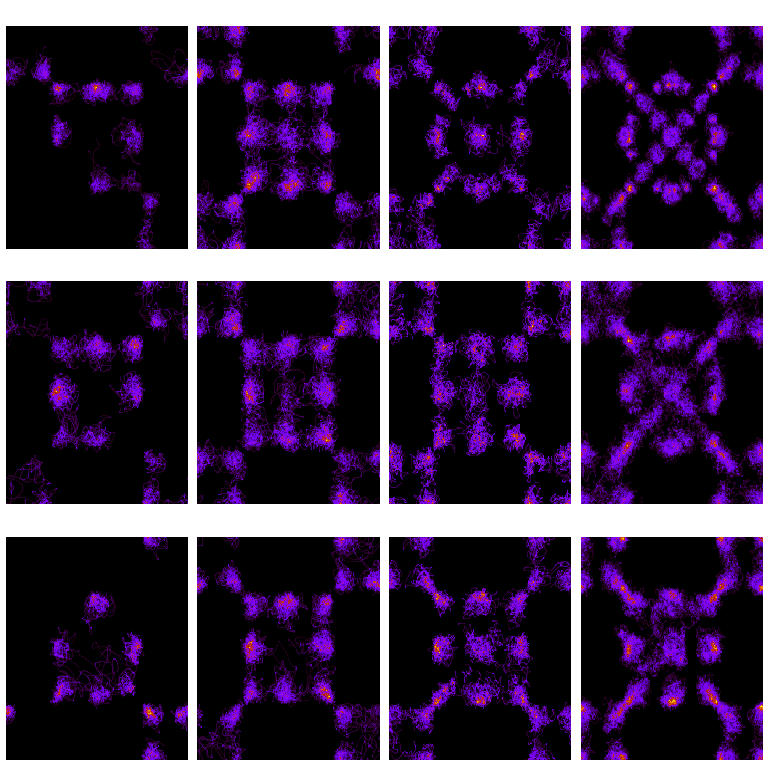
\includegraphics{zif8x-density}}%
    \gplfronttext
  \end{picture}%
\endgroup

    \caption{Cartes de densité 2D de l'azote adsorbé dans le plan $xy$
    à divers remplissages dans \ZIFCH3 (haut), \ZIFCl (milieu), et \ZIFBr
    (bas).}
    \label{fig:fr:zif8x:density}
\end{figure}

Une autre hypothèse que nous pouvons formuler pour expliquer la présence du
second saut dans les isothermes est que les molécules d'azote subissent une
ré-organisation dans les pores, entraînant ainsi une augmentation du nombre de
molécules adsorbées dans un volume poreux constant ainsi que la rotation des
ligands. Afin de visualiser l'organisation des molécules, j'ai projeté les
positions de tous les atomes d'azote adsorbés dans le plan $xy$ et créé une
carte de densité de la phase adsorbée. Cette carte de densité est présentée
figure~\ref{fig:fr:zif8x:density}, pour différents remplissages et pour les trois
structures.

Pour \ZIFCH3, on rencontre deux organisations moléculaires différentes en
fonction du remplissage. Avec 10 ou 25 molécules par maille, les cartes de
densité montrent des positions clairement délimitées sur un arrangement cubique,
tandis qu'avec 40 et 50 molécules, elles montrent un arrangement tétragonal de
ces mêmes molécules. Pour \ZIFCl, le comportement est à peu près similaire: les
molécules s'organisent d'abord de façon cubique lorsqu'il y a 10, 25 et 40
molécules par mailles, avant de se réordonner vers un arrangement tétragonal à
50 molécules par mailles.

Ceci est cohérent avec les distributions des angles dièdres en
figure~\ref{fig:zif8x:dihedrals}, et la preuve que le réarrangement des
molécules d'azote se produit conjointement avec la rotation des ligands. Il est
intéressant de noter qu'un certain désordre dans l'arrangement tétragonal reste
présent --- même à un remplissage de 50 molécules par maille --- les positions
des molécules n'étant pas aussi bien définies que dans la \ZIFCH3. Encore une
fois, ceci est cohérent avec la distribution des angles dièdres pour un
remplissage de 50 molécules par mailles pour \ZIFCl qui n'est pas de type
gaussien, indiquant que ce désordre se retrouve aussi dans la structure. Pour
\ZIFBr, le comportement est différent. On trouve le même agencement cubique aux
remplissages de 8 et 20 molécules par mailles, alors que l'agencement pour 40 et
50 molécules par mailles n'est pas le même que celui observé dans la \ZIFCH3 et
\ZIFCl. Les molécules semblent être principalement réparties sur un cube avec
des molécules supplémentaires sur les diagonales du cube.

Le mécanisme que je propose pour l'adsorption de l'azote dans les trois
structures \ZIF8 est illustré schématiquement en figure~\ref{fig:zif8x:summary}.
Lorsque les pores sont vides, les ligands sont dans leur position d'équilibre,
autour de 0°. Au fur et à mesure que le remplissage augmente, les pores se
remplissent selon un agencement cubique. Puis, comme le remplissage continue à
augmenter, les molécules se ré-arrangent dans \ZIFCH3 et \ZIFCl pour passer à un
arrangement tétragonal. La rotation des ligands accompagne ce ré-arrangement des
molécules. Aucun de ces deux phénomènes n'a lieu dans \ZIFBr, sans doutes à cause
des différences de taille et de forme des pores, les pores de \ZIFBr étant
plus petits que ceux de \ZIFCl et de \ZIFCH3.

\clearpage
\section{Champs de force à partir de données \abinitio}

Pendant ma thèse, j'ai également collaboré avec Johannes Dürholt et Rochus
Schmid de la Ruhr Universität à Bochum en Allemagne. Nous avons paramétré un
champ de force classique pour \ZIFCH3, \ZIFCl et \ZIFBr en utilisant les
simulations \abinitio présentées précédemment. L'article correspondant est
publié dans \citejournal{Duerholt2019}\cite{Duerholt2019}.

Idéalement, nous aimerions que les champs de force que nous utilisons soient
aussi précis que possible lors du calcul de l'énergie d'un système, afin d'être
aussi sûrs que possible que le modèle décrit par le champ de force décrive la
réalité chimique. Cela nous impose de créer un champ de force spécifique pour
chaque molécule et pour chaque combinaison de molécules. Cependant, le fait
d'avoir des champs de force distincts pour chaque système peut nous empêcher de
comparer les propriétés prédites par les simulations. Nous ne pouvons pas
attribuer avec certitude les différences de prédiction à la réalité chimique
sous-jacente, et non au modèle utilisé. C'est la raison pour laquelle des champs
de force génériques ont également été développés. Ils sacrifient un peu de
précision pour plus transférables: ces champs de forces sont utilisables pour de
multiples systèmes moléculaires avec à peu près la même précision partout.
Malheureusement, les champs de force génériques existants ne sont pas toujours
optimaux pour simuler les MOF, principalement en raison des liens de
coordination existant entre les centres métalliques et les lieurs organiques.

Une façon de surmonter ces problèmes (temps de paramétrage long, compromis entre
champs de force transférables et champs de force précis) est d'utiliser un
algorithme de paramétrisation systématique. L'utilisation du même algorithme
pour tous les systèmes d'intérêt permet d'améliorer la précision, car chaque
système a des paramètres qui lui sont propres, tout en permettant la comparaison
entre différents systèmes, car ils partagent la même forme fonctionnelle et les
mêmes données de référence. Plusieurs approches ont été développées pour générer
de nouveaux champs de forces pour les MOF, telles que
Quick-FF\cite{Vanduyfhuys2015} et MOF-FF\cite{Bureekaew2013}. Les deux utilisent
des données de référence \abinitio, telles que la géométrie optimisée, et la
matrice Hessienne du système. Pour optimiser les paramètres du champ de force,
ils utilisent des algorithmes d'apprentissage machine, tels que des algorithmes
génétiques.

Johannes Dürholt a utilisé MOF-FF pour générer de nouveaux champs de force pour
\ZIFCH3, \ZIFCl, et \ZIFBr à partir des données de référence \abinitio. J'ai
contribué à ce travail en fournissant les simulations de ZIF vides décrites
précédemment et en aidant à l'analyse des trajectoires afin de valider le champ
de force. Les versions précédentes de MOF-FF utilisaient des clusters finis
représentatifs dans le vide pour paramétrer le champs de force. Au cours de ces
travaux, la stratégie d'ajustement des paramètres a été améliorée pour permettre
l'utilisation de conditions aux limites périodiques. Il n'est donc plus
nécessaire de trouver des clusters finis représentatifs et non chargés, ce qui
n'est pas toujours possible en fonction de la topologie du MOF considéré.  Les
champs de force ainsi généré sont capable de reproduire non seulement les
propriétés géométriques statiques des trois ZIFs, mais aussi certaines
propriétés dynamiques comme les modes de vibration ou globales comme les
coefficients d'élasticité (voir la figure~\ref{fig:fig:mof-ff:validation} et les
tables~\ref{tab:mof-ff:unit-cell} et~\ref{tab:mof-ff:elastic}).

\clearpage
\section{Intrusion d'électrolytes dans la \ZIF8}

L'intrusion de liquides non mouillants, et en particulier du mercure, est
utilisée depuis longtemps pour caractériser les matériaux poreux ayant des
largeurs de pores comprises entre \SI{50}{nm}{nm} et
\SI{500}{\um}\cite{Rouquerol2011}. L'intrusion peut être vue comme une
adsorption de fluides au-dessus de la pression de vapeur saturante, c'est-à-dire
quand le fluide est dans son état liquide. Depuis les années 2000, le mouillage
forcé des solutions électrolytiques a été étudié, révélant des effets très
intéressants de pression osmotique géante\cite{Liu2009, MichelinJamois2015}, et
des applications potentielles pour le stockage et la dissipation de l'énergie
mécanique\cite{Eroshenko2001}. Les lecteurs intéressés peuvent consulter la
revue de littérature que j'ai aidé à écrire sur le sujet, publiée dans
\citejournal{Fraux2017-2}\cite{Fraux2017-2}. L'utilisation d'ions dans le
liquide d'intrusion permet non seulement de modifier la pression d'intrusion par
des effets osmotiques\cite{Tzanis2014, Khay2014}, mais aussi de changer la forme
de l'isotherme d'intrusion, passant d'un comportement de stockage de l'énergie à
la dissipation de cette énergie\cite{Ryzhikov2014}.

Au cours de ma thèse, j'ai étudié l'intrusion haute pression d'électrolyte dans
la \ZIF8. Ce matériau \ZIF8 est hydrophobe\cite{AOrtiz2014} et présente un
comportement intéressant pendant d'intrusion. Alors que les effets de pression
osmotique ne dépendent pas de la nature chimique des ions mais seulement de leur
concentration, la \ZIF8 passe d'un comportement énergétique à l'autre lorsque la
nature ionique change à concentration constante\cite{Ortiz2014}. Le mécanisme
exact et le comportement au niveau moléculaire de l'intrusion d'électrolytes
dans la \ZIF8 sont encore inconnus. J'ai utilisé des simulations de dynamique
moléculaires classiques pour étudier la structure, la dynamique et les
implications énergétiques du confinement de l'eau et des solutions aqueuses de
LiCl dans la \ZIF8. Pour ce faire, j'ai réalisé des simulations d'eau libre et
confinée à différentes pressions (de 0 à \SI{1}{Gpa}) et avec différentes
concentrations d'ions (de 0 à \SI{20}{mol/L}).

Du point de vue du liquide, le principal effet de l'intrusion est le confinement
du fluide dans un espace poreux de dimensions nanométriques. Afin de
caractériser la structure du liquide et la solvatation des ions, j'ai calculé le
nombre de voisins dans la première couche de solvatation
(figure~\ref{fig:licl-zif:neighbors}) et des cartes de densité 2D pour la
répartition des molécules dans le pore (figure~\ref{fig:licl-zif:density}). Sur
ces figures, on peut observer que le confinement modifie la structure de l'eau
et la solvatation des ions, créant une structuration à longue distance du réseau
de liaisons hydrogène. Les molécules d'eau occupent des sites très bien définis,
notamment à l'intérieur des fenêtres entre deux cages voisines. Au fur et à
mesure que la concentration augmente, cette organisation est légèrement
perturbée par les ions insérés dans le réseau des molécules d'eau. La présence
de la \ZIF8 empêche aussi l'eau de se ré-organiser, et diminue donc la
solvatation des ions à haute concentration, quand il n'y a plus assez de
molécules d'eau pour chaque ion.

J'ai caractérisé la dynamique de l'eau via celle des liaisons hydrogène. J'ai
considéré qu'une liaison hydrogène était présente entre deux molécules d'eau si
les deux atomes d'oxygène sont séparés par moins de \SI{3.5}{\AA}, avec un
angle oxygène-oxygène-hydrogène ($\widehat{\text{OOH}}$) inférieur à 30°. J'ai
ensuite calculé l'auto-corrélation temporelle des fonctions d'existence de la
liaison hydrogène $H(t)$ --- qui vaut 1 si la liaison existe au temps $t$, 0 si
elle n'existe pas:
\[C_{\text{hbonds}}(t) = \left\langle H(t_0) \cdot H(t_0 + t) \right\rangle_{t_0}. \]
La décroissance de cette fonction d'auto-corrélation est caractéristique de la
dynamique du réseau de liaisons hydrogène et de la constante de temps des liaisons
hydrogène individuelles. Cette décroissance n'est pas décrite adéquatement par
un modèle exponentiel pur, c'est pourquoi j'ai utilisé un modèle bi-exponentiel
pour extraire les constantes de temps:
\[ f(t) = A_1 e^{-t / \tau_1} + A_2 e^{-t / \tau_2}.\]
où $\tau_1$ et $\tau_2$ sont les deux constantes de temps de la décroissance, et
$A_1$ et $A_2$ sont leur poids relatif. Les paramètres d'ajustement résultants
sont présentés dans table~\ref{table:licl-zif:hbonds} et
figure~\ref{fig:fr:licl-zif:hbonds:fit:pressure}.

\begin{figure}[ht]
    \centering
    % GNUPLOT: LaTeX picture with Postscript
\begingroup
  \makeatletter
  \providecommand\color[2][]{%
    \GenericError{(gnuplot) \space\space\space\@spaces}{%
      Package color not loaded in conjunction with
      terminal option `colourtext'%
    }{See the gnuplot documentation for explanation.%
    }{Either use 'blacktext' in gnuplot or load the package
      color.sty in LaTeX.}%
    \renewcommand\color[2][]{}%
  }%
  \providecommand\includegraphics[2][]{%
    \GenericError{(gnuplot) \space\space\space\@spaces}{%
      Package graphicx or graphics not loaded%
    }{See the gnuplot documentation for explanation.%
    }{The gnuplot epslatex terminal needs graphicx.sty or graphics.sty.}%
    \renewcommand\includegraphics[2][]{}%
  }%
  \providecommand\rotatebox[2]{#2}%
  \@ifundefined{ifGPcolor}{%
    \newif\ifGPcolor
    \GPcolortrue
  }{}%
  \@ifundefined{ifGPblacktext}{%
    \newif\ifGPblacktext
    \GPblacktextfalse
  }{}%
  % define a \g@addto@macro without @ in the name:
  \let\gplgaddtomacro\g@addto@macro
  % define empty templates for all commands taking text:
  \gdef\gplbacktext{}%
  \gdef\gplfronttext{}%
  \makeatother
  \ifGPblacktext
    % no textcolor at all
    \def\colorrgb#1{}%
    \def\colorgray#1{}%
  \else
    % gray or color?
    \ifGPcolor
      \def\colorrgb#1{\color[rgb]{#1}}%
      \def\colorgray#1{\color[gray]{#1}}%
      \expandafter\def\csname LTw\endcsname{\color{white}}%
      \expandafter\def\csname LTb\endcsname{\color{black}}%
      \expandafter\def\csname LTa\endcsname{\color{black}}%
      \expandafter\def\csname LT0\endcsname{\color[rgb]{1,0,0}}%
      \expandafter\def\csname LT1\endcsname{\color[rgb]{0,1,0}}%
      \expandafter\def\csname LT2\endcsname{\color[rgb]{0,0,1}}%
      \expandafter\def\csname LT3\endcsname{\color[rgb]{1,0,1}}%
      \expandafter\def\csname LT4\endcsname{\color[rgb]{0,1,1}}%
      \expandafter\def\csname LT5\endcsname{\color[rgb]{1,1,0}}%
      \expandafter\def\csname LT6\endcsname{\color[rgb]{0,0,0}}%
      \expandafter\def\csname LT7\endcsname{\color[rgb]{1,0.3,0}}%
      \expandafter\def\csname LT8\endcsname{\color[rgb]{0.5,0.5,0.5}}%
    \else
      % gray
      \def\colorrgb#1{\color{black}}%
      \def\colorgray#1{\color[gray]{#1}}%
      \expandafter\def\csname LTw\endcsname{\color{white}}%
      \expandafter\def\csname LTb\endcsname{\color{black}}%
      \expandafter\def\csname LTa\endcsname{\color{black}}%
      \expandafter\def\csname LT0\endcsname{\color{black}}%
      \expandafter\def\csname LT1\endcsname{\color{black}}%
      \expandafter\def\csname LT2\endcsname{\color{black}}%
      \expandafter\def\csname LT3\endcsname{\color{black}}%
      \expandafter\def\csname LT4\endcsname{\color{black}}%
      \expandafter\def\csname LT5\endcsname{\color{black}}%
      \expandafter\def\csname LT6\endcsname{\color{black}}%
      \expandafter\def\csname LT7\endcsname{\color{black}}%
      \expandafter\def\csname LT8\endcsname{\color{black}}%
    \fi
  \fi
    \setlength{\unitlength}{0.0500bp}%
    \ifx\gptboxheight\undefined%
      \newlength{\gptboxheight}%
      \newlength{\gptboxwidth}%
      \newsavebox{\gptboxtext}%
    \fi%
    \setlength{\fboxrule}{0.5pt}%
    \setlength{\fboxsep}{1pt}%
\begin{picture}(7580.00,5100.00)%
    \gplgaddtomacro\gplbacktext{%
      \csname LTb\endcsname%%
      \put(408,2667){\makebox(0,0)[r]{\strut{}$0$}}%
      \csname LTb\endcsname%%
      \put(408,3037){\makebox(0,0)[r]{\strut{}$1$}}%
      \csname LTb\endcsname%%
      \put(408,3408){\makebox(0,0)[r]{\strut{}$2$}}%
      \csname LTb\endcsname%%
      \put(408,3778){\makebox(0,0)[r]{\strut{}$3$}}%
      \csname LTb\endcsname%%
      \put(408,4148){\makebox(0,0)[r]{\strut{}$4$}}%
      \csname LTb\endcsname%%
      \put(510,2481){\makebox(0,0){\strut{}$0$}}%
      \csname LTb\endcsname%%
      \put(1253,2481){\makebox(0,0){\strut{}$5$}}%
      \csname LTb\endcsname%%
      \put(1997,2481){\makebox(0,0){\strut{}$10$}}%
      \csname LTb\endcsname%%
      \put(2740,2481){\makebox(0,0){\strut{}$15$}}%
      \csname LTb\endcsname%%
      \put(3483,2481){\makebox(0,0){\strut{}$20$}}%
    }%
    \gplgaddtomacro\gplfronttext{%
      \csname LTb\endcsname%%
      \put(120,3407){\rotatebox{-270}{\makebox(0,0){\strut{}$\tau_1$ (ps)}}}%
      \csname LTb\endcsname%%
      \put(1137,4440){\makebox(0,0){\strut{}\footnotesize 0}}%
      \csname LTb\endcsname%%
      \put(1768,4440){\makebox(0,0){\strut{}\footnotesize 0.33}}%
      \csname LTb\endcsname%%
      \put(2399,4440){\makebox(0,0){\strut{}\footnotesize 0.67}}%
      \csname LTb\endcsname%%
      \put(3031,4440){\makebox(0,0){\strut{}\footnotesize 1}}%
      \csname LTb\endcsname%%
      \put(2084,5016){\makebox(0,0){\strut{}\footnotesize bulk liquid pressure (GPa)}}%
    }%
    \gplgaddtomacro\gplbacktext{%
      \csname LTb\endcsname%%
      \put(4198,2667){\makebox(0,0)[r]{\strut{}$0$}}%
      \csname LTb\endcsname%%
      \put(4198,3037){\makebox(0,0)[r]{\strut{}$25$}}%
      \csname LTb\endcsname%%
      \put(4198,3408){\makebox(0,0)[r]{\strut{}$50$}}%
      \csname LTb\endcsname%%
      \put(4198,3778){\makebox(0,0)[r]{\strut{}$75$}}%
      \csname LTb\endcsname%%
      \put(4198,4148){\makebox(0,0)[r]{\strut{}$100$}}%
      \csname LTb\endcsname%%
      \put(4300,2481){\makebox(0,0){\strut{}$0$}}%
      \csname LTb\endcsname%%
      \put(5043,2481){\makebox(0,0){\strut{}$5$}}%
      \csname LTb\endcsname%%
      \put(5787,2481){\makebox(0,0){\strut{}$10$}}%
      \csname LTb\endcsname%%
      \put(6530,2481){\makebox(0,0){\strut{}$15$}}%
      \csname LTb\endcsname%%
      \put(7273,2481){\makebox(0,0){\strut{}$20$}}%
    }%
    \gplgaddtomacro\gplfronttext{%
      \csname LTb\endcsname%%
      \put(3808,3407){\rotatebox{-270}{\makebox(0,0){\strut{}$\tau_2$ (ps)}}}%
    }%
    \gplgaddtomacro\gplbacktext{%
      \csname LTb\endcsname%%
      \put(408,627){\makebox(0,0)[r]{\strut{}$0$}}%
      \csname LTb\endcsname%%
      \put(408,998){\makebox(0,0)[r]{\strut{}$25$}}%
      \csname LTb\endcsname%%
      \put(408,1368){\makebox(0,0)[r]{\strut{}$50$}}%
      \csname LTb\endcsname%%
      \put(408,1739){\makebox(0,0)[r]{\strut{}$75$}}%
      \csname LTb\endcsname%%
      \put(408,2109){\makebox(0,0)[r]{\strut{}$100$}}%
      \csname LTb\endcsname%%
      \put(510,441){\makebox(0,0){\strut{}$0$}}%
      \csname LTb\endcsname%%
      \put(1253,441){\makebox(0,0){\strut{}$5$}}%
      \csname LTb\endcsname%%
      \put(1997,441){\makebox(0,0){\strut{}$10$}}%
      \csname LTb\endcsname%%
      \put(2740,441){\makebox(0,0){\strut{}$15$}}%
      \csname LTb\endcsname%%
      \put(3483,441){\makebox(0,0){\strut{}$20$}}%
    }%
    \gplgaddtomacro\gplfronttext{%
      \csname LTb\endcsname%%
      \put(69,1368){\rotatebox{-270}{\makebox(0,0){\strut{}$A_1$ (\%)}}}%
      \csname LTb\endcsname%%
      \put(1996,162){\makebox(0,0){\strut{}\footnotesize concentration (mol/L)}}%
    }%
    \gplgaddtomacro\gplbacktext{%
      \csname LTb\endcsname%%
      \put(4198,627){\makebox(0,0)[r]{\strut{}$0$}}%
      \csname LTb\endcsname%%
      \put(4198,998){\makebox(0,0)[r]{\strut{}$25$}}%
      \csname LTb\endcsname%%
      \put(4198,1368){\makebox(0,0)[r]{\strut{}$50$}}%
      \csname LTb\endcsname%%
      \put(4198,1739){\makebox(0,0)[r]{\strut{}$75$}}%
      \csname LTb\endcsname%%
      \put(4198,2109){\makebox(0,0)[r]{\strut{}$100$}}%
      \csname LTb\endcsname%%
      \put(4300,441){\makebox(0,0){\strut{}$0$}}%
      \csname LTb\endcsname%%
      \put(5043,441){\makebox(0,0){\strut{}$5$}}%
      \csname LTb\endcsname%%
      \put(5787,441){\makebox(0,0){\strut{}$10$}}%
      \csname LTb\endcsname%%
      \put(6530,441){\makebox(0,0){\strut{}$15$}}%
      \csname LTb\endcsname%%
      \put(7273,441){\makebox(0,0){\strut{}$20$}}%
    }%
    \gplgaddtomacro\gplfronttext{%
      \csname LTb\endcsname%%
      \put(3808,1368){\rotatebox{-270}{\makebox(0,0){\strut{}$A_2$ (\%)}}}%
      \csname LTb\endcsname%%
      \put(5786,162){\makebox(0,0){\strut{}\footnotesize concentration (mol/L)}}%
    }%
    \gplgaddtomacro\gplbacktext{%
    }%
    \gplgaddtomacro\gplfronttext{%
      \csname LTb\endcsname%%
      \put(4926,4440){\makebox(0,0){\strut{}\footnotesize 0}}%
      \csname LTb\endcsname%%
      \put(5557,4440){\makebox(0,0){\strut{}\footnotesize 0.33}}%
      \csname LTb\endcsname%%
      \put(6188,4440){\makebox(0,0){\strut{}\footnotesize 0.67}}%
      \csname LTb\endcsname%%
      \put(6820,4440){\makebox(0,0){\strut{}\footnotesize 1}}%
      \csname LTb\endcsname%%
      \put(5873,5016){\makebox(0,0){\strut{}\footnotesize confined liquid pressure (GPa)}}%
    }%
    \gplgaddtomacro\gplbacktext{%
    }%
    \gplgaddtomacro\gplfronttext{%
    }%
    \gplgaddtomacro\gplbacktext{%
    }%
    \gplgaddtomacro\gplfronttext{%
    }%
    \gplgaddtomacro\gplbacktext{%
    }%
    \gplgaddtomacro\gplfronttext{%
    }%
    \gplbacktext
    \put(0,0){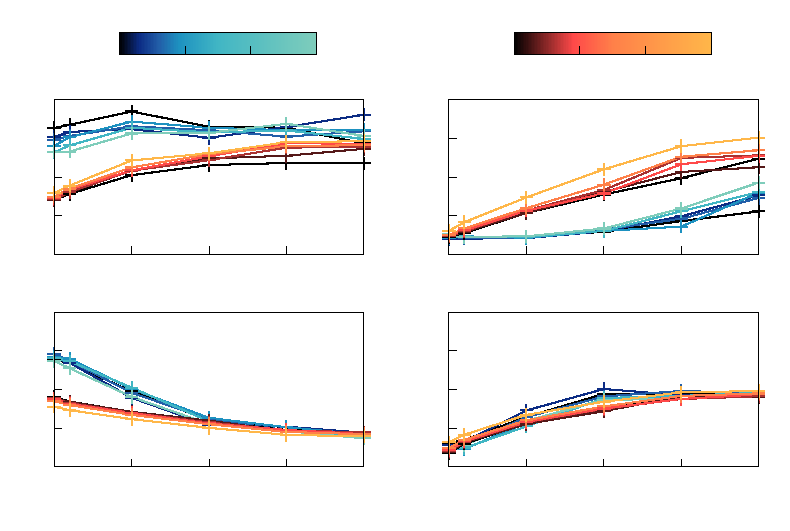
\includegraphics{licl-zif-hbonds-fit-pressure}}%
    \gplfronttext
  \end{picture}%
\endgroup

    \caption{Variations de la constante de temps et de la proportion des deux
    termes exponentiels dans l'auto-corrélation de liaisons hydrogène en fonction
    de la pression et de la concentration en ions dans les liquides purs
    (teintes bleues) et confinés (teintes rouges).}
    \label{fig:fr:licl-zif:hbonds:fit:pressure}
\end{figure}

Tout d'abord, nous remarquons que la pression a une influence relativement
faible sur la dynamique des liaisons hydrogène. Dans le liquide pur, la
constante de temps la plus courte est relativement constante autour de
\SI{3}{ps} lorsque la concentration augmente, mais le poids de ce processus
rapide ($A_1$) diminue. Cela suggère que cette constante de temps rapide est
associée à des liaisons hydrogène entre molécules d'eau entourées seulement par
d'autres molécules d'eau. La deuxième constante de temps, associée au processus
le plus lent, augmente avec la concentration, ainsi que le poids correspondant
($A_2$). Cela indique des liaisons hydrogène entre les molécules d'eau liées aux
ions. Dans le liquide confiné, les poids évoluent de la même façon par rapport à
la concentration, ce qui indique qu'ils sont associés au même type de liaisons
hydrogène que dans le liquide pur. La deuxième constante de temps augmente dans
le liquide confiné par rapport au liquide pur. Ce ralentissement de la
dynamique de l'eau en confinement est bien connue\cite{Fogarty2014}, et a été
observé dans de nombreuses classes de matériaux nanoporeux\cite{Jeffery2004,
RomeroVargasCastrillon2009, Haigis2013, Scalfi2018}.

J'ai également étudié la thermodynamique du processus par lequel des molécules
d'eau et des ions peuvent entrer dans les pores de la \ZIF8 en passant par les
fenêtres à 6 membres. J'ai donc modélisé une interface eau/\ZIF8 explicite,
représentée dans la figure~\ref{fig:licl-zif:umbrella-system}: le système
contient à la fois de l'eau pure et de l'eau confinée dans la \ZIF8. J'ai
utilisé des simulations \emph{umbrella sampling} et la méthode d'analyse WHAM
pour reconstruire le profil d'énergie libre des molécules (\ce{Li+}, \ce{Cl-},
ou \ce{H2O}) entrant \ZIF8 selon l'axe cristallographique (111), reproduit en
figure~\ref{fig:fr:licl-zif:free}.

\begin{figure}[ht]
    \vskip-1ex
    \centering
    % GNUPLOT: LaTeX picture with Postscript
\begingroup
  \makeatletter
  \providecommand\color[2][]{%
    \GenericError{(gnuplot) \space\space\space\@spaces}{%
      Package color not loaded in conjunction with
      terminal option `colourtext'%
    }{See the gnuplot documentation for explanation.%
    }{Either use 'blacktext' in gnuplot or load the package
      color.sty in LaTeX.}%
    \renewcommand\color[2][]{}%
  }%
  \providecommand\includegraphics[2][]{%
    \GenericError{(gnuplot) \space\space\space\@spaces}{%
      Package graphicx or graphics not loaded%
    }{See the gnuplot documentation for explanation.%
    }{The gnuplot epslatex terminal needs graphicx.sty or graphics.sty.}%
    \renewcommand\includegraphics[2][]{}%
  }%
  \providecommand\rotatebox[2]{#2}%
  \@ifundefined{ifGPcolor}{%
    \newif\ifGPcolor
    \GPcolortrue
  }{}%
  \@ifundefined{ifGPblacktext}{%
    \newif\ifGPblacktext
    \GPblacktextfalse
  }{}%
  % define a \g@addto@macro without @ in the name:
  \let\gplgaddtomacro\g@addto@macro
  % define empty templates for all commands taking text:
  \gdef\gplbacktext{}%
  \gdef\gplfronttext{}%
  \makeatother
  \ifGPblacktext
    % no textcolor at all
    \def\colorrgb#1{}%
    \def\colorgray#1{}%
  \else
    % gray or color?
    \ifGPcolor
      \def\colorrgb#1{\color[rgb]{#1}}%
      \def\colorgray#1{\color[gray]{#1}}%
      \expandafter\def\csname LTw\endcsname{\color{white}}%
      \expandafter\def\csname LTb\endcsname{\color{black}}%
      \expandafter\def\csname LTa\endcsname{\color{black}}%
      \expandafter\def\csname LT0\endcsname{\color[rgb]{1,0,0}}%
      \expandafter\def\csname LT1\endcsname{\color[rgb]{0,1,0}}%
      \expandafter\def\csname LT2\endcsname{\color[rgb]{0,0,1}}%
      \expandafter\def\csname LT3\endcsname{\color[rgb]{1,0,1}}%
      \expandafter\def\csname LT4\endcsname{\color[rgb]{0,1,1}}%
      \expandafter\def\csname LT5\endcsname{\color[rgb]{1,1,0}}%
      \expandafter\def\csname LT6\endcsname{\color[rgb]{0,0,0}}%
      \expandafter\def\csname LT7\endcsname{\color[rgb]{1,0.3,0}}%
      \expandafter\def\csname LT8\endcsname{\color[rgb]{0.5,0.5,0.5}}%
    \else
      % gray
      \def\colorrgb#1{\color{black}}%
      \def\colorgray#1{\color[gray]{#1}}%
      \expandafter\def\csname LTw\endcsname{\color{white}}%
      \expandafter\def\csname LTb\endcsname{\color{black}}%
      \expandafter\def\csname LTa\endcsname{\color{black}}%
      \expandafter\def\csname LT0\endcsname{\color{black}}%
      \expandafter\def\csname LT1\endcsname{\color{black}}%
      \expandafter\def\csname LT2\endcsname{\color{black}}%
      \expandafter\def\csname LT3\endcsname{\color{black}}%
      \expandafter\def\csname LT4\endcsname{\color{black}}%
      \expandafter\def\csname LT5\endcsname{\color{black}}%
      \expandafter\def\csname LT6\endcsname{\color{black}}%
      \expandafter\def\csname LT7\endcsname{\color{black}}%
      \expandafter\def\csname LT8\endcsname{\color{black}}%
    \fi
  \fi
    \setlength{\unitlength}{0.0500bp}%
    \ifx\gptboxheight\undefined%
      \newlength{\gptboxheight}%
      \newlength{\gptboxwidth}%
      \newsavebox{\gptboxtext}%
    \fi%
    \setlength{\fboxrule}{0.5pt}%
    \setlength{\fboxsep}{1pt}%
\begin{picture}(5660.00,5660.00)%
    \gplgaddtomacro\gplbacktext{%
      \csname LTb\endcsname%%
      \put(752,3264){\makebox(0,0)[r]{\strut{}$-10$}}%
      \csname LTb\endcsname%%
      \put(752,3627){\makebox(0,0)[r]{\strut{}$0$}}%
      \csname LTb\endcsname%%
      \put(752,3990){\makebox(0,0)[r]{\strut{}$10$}}%
      \csname LTb\endcsname%%
      \put(752,4353){\makebox(0,0)[r]{\strut{}$20$}}%
      \csname LTb\endcsname%%
      \put(752,4716){\makebox(0,0)[r]{\strut{}$30$}}%
      \csname LTb\endcsname%%
      \put(752,5079){\makebox(0,0)[r]{\strut{}$40$}}%
      \csname LTb\endcsname%%
      \put(752,5442){\makebox(0,0)[r]{\strut{}$50$}}%
      \csname LTb\endcsname%%
      \put(871,3047){\makebox(0,0){\strut{}$-20$}}%
      \csname LTb\endcsname%%
      \put(1425,3047){\makebox(0,0){\strut{}$-15$}}%
      \csname LTb\endcsname%%
      \put(1979,3047){\makebox(0,0){\strut{}$-10$}}%
      \csname LTb\endcsname%%
      \put(2533,3047){\makebox(0,0){\strut{}$-5$}}%
      \csname LTb\endcsname%%
      \put(3087,3047){\makebox(0,0){\strut{}$0$}}%
      \csname LTb\endcsname%%
      \put(3640,3047){\makebox(0,0){\strut{}$5$}}%
      \csname LTb\endcsname%%
      \put(4194,3047){\makebox(0,0){\strut{}$10$}}%
      \csname LTb\endcsname%%
      \put(4748,3047){\makebox(0,0){\strut{}$15$}}%
      \csname LTb\endcsname%%
      \put(5302,3047){\makebox(0,0){\strut{}$20$}}%
    }%
    \gplgaddtomacro\gplfronttext{%
      \csname LTb\endcsname%%
      \put(178,4353){\rotatebox{-270}{\makebox(0,0){\strut{}free energy (kcal/mol)}}}%
      \csname LTb\endcsname%%
      \put(2924,5247){\makebox(0,0)[r]{\strut{}\ce{Li}}}%
      \csname LTb\endcsname%%
      \put(2924,5030){\makebox(0,0)[r]{\strut{}\ce{Cl}}}%
      \csname LTb\endcsname%%
      \put(2924,4813){\makebox(0,0)[r]{\strut{}\ce{H2O}}}%
    }%
    \gplgaddtomacro\gplbacktext{%
      \csname LTb\endcsname%%
      \put(633,694){\makebox(0,0)[r]{\strut{}$0$}}%
      \csname LTb\endcsname%%
      \put(633,1078){\makebox(0,0)[r]{\strut{}$2$}}%
      \csname LTb\endcsname%%
      \put(633,1462){\makebox(0,0)[r]{\strut{}$4$}}%
      \csname LTb\endcsname%%
      \put(633,1845){\makebox(0,0)[r]{\strut{}$6$}}%
      \csname LTb\endcsname%%
      \put(633,2229){\makebox(0,0)[r]{\strut{}$8$}}%
      \csname LTb\endcsname%%
      \put(633,2613){\makebox(0,0)[r]{\strut{}$10$}}%
      \csname LTb\endcsname%%
      \put(752,477){\makebox(0,0){\strut{}$-20$}}%
      \csname LTb\endcsname%%
      \put(1321,477){\makebox(0,0){\strut{}$-15$}}%
      \csname LTb\endcsname%%
      \put(1890,477){\makebox(0,0){\strut{}$-10$}}%
      \csname LTb\endcsname%%
      \put(2458,477){\makebox(0,0){\strut{}$-5$}}%
      \csname LTb\endcsname%%
      \put(3027,477){\makebox(0,0){\strut{}$0$}}%
      \csname LTb\endcsname%%
      \put(3596,477){\makebox(0,0){\strut{}$5$}}%
      \csname LTb\endcsname%%
      \put(4165,477){\makebox(0,0){\strut{}$10$}}%
      \csname LTb\endcsname%%
      \put(4733,477){\makebox(0,0){\strut{}$15$}}%
      \csname LTb\endcsname%%
      \put(5302,477){\makebox(0,0){\strut{}$20$}}%
    }%
    \gplgaddtomacro\gplfronttext{%
      \csname LTb\endcsname%%
      \put(178,1653){\rotatebox{-270}{\makebox(0,0){\strut{}number of neighbors}}}%
      \csname LTb\endcsname%%
      \put(3027,152){\makebox(0,0){\strut{}x ($\AA$)}}%
    }%
    \gplbacktext
    \put(0,0){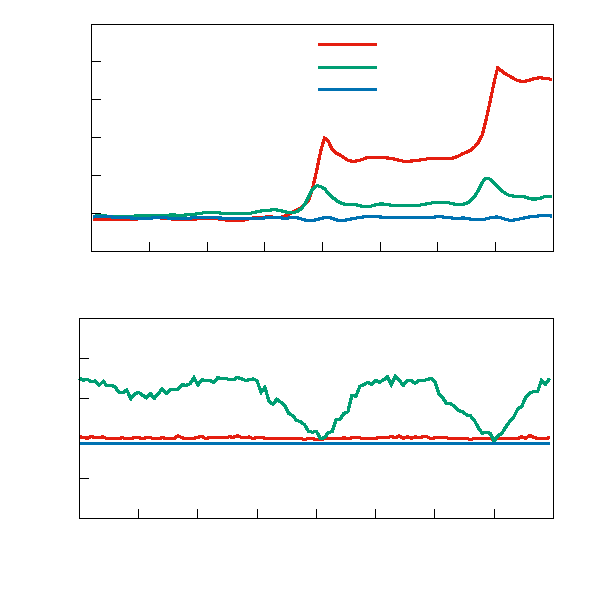
\includegraphics{licl-zif-free-energy}}%
    \gplfronttext
  \end{picture}%
\endgroup

    \vskip-2ex
    \caption{(haut) Profil d'énergie libre d'une molécule entrant dans la \ZIF8
    et nombre correspondant de voisins (bas) dans la première couche de
    solvatation en fonction de la position de la molécule sur l'axe
    cristallographique (111). La première fenêtre de la \ZIF8 est à $x=0$ ;
    la zone $x<0$ correspond à l'eau pure, et la zone $x>0$ à l'eau confinée
    dans la \ZIF8.}
    \vskip-1ex
    \label{fig:fr:licl-zif:free}
\end{figure}

Tout d'abord, on peut remarquer que les molécules d'eau entre dans la \ZIF8 sans
la moindre barrière. Pour les anions chlorure, nous observons deux barrières sur
le profil d'énergie libre, qui correspondent aux fenêtres de la \ZIF8 à 0 et
\SI{15}{\AA}. Ces barrières sont corrélées à un nombre inférieur de voisins pour
l'ion: l'anion doit se désolvater partiellement pour passer à travers la
fenêtre, ce qui explique la barrière d'énergie libre. En dehors de ces
barrières, le profil est plat et au même niveau que dans le liquide pur: les
ions \ce{Cl-} ont une barrière cinétique à l'entrée dans le \ZIF8, mais pas de
barrière thermodynamique. Les résultats pour Li sont plus surprenants. Nous
voyons à la fois une barrière élevée à la première ($x=\SI{0}{\AA}$) et à la
deuxième ($x=\SI{15}{\AA}$) fenêtre; et une différence énergétique entre
l'extérieur et l'intérieur des pores valant approximativement \SI{15}{kcal/mol}.
Cette différence d'énergie n'est pas seulement due à la transition entre le
liquide pur et le liquide confiné, car elle est également présente au niveau de
la deuxième fenêtre. En même temps, ces barrières ne sont pas liées à une
différence de solvatation comme dans le cas du chlore. Ceci indique une
différence de nature entre les ions \ce{Li+} et \ce{Cl-}, qui devront être
approfondis.

\clearpage
\section{Adsorption d'eau dans les imogolites}

J'ai aussi étudié l'adsorption d'eau dans un matériau hydrophile: l'imogolite.
Il s'agit de nanotubes d'aluminosilicate dont la structure est représentée en
figure~\ref{fig:imogolite:structure}. J'ai pour cela collaboré avec Laura Scalfi
durant son stage de master. Nous avons utilisé des simulations Monte-Carlo grand
canonique et la dynamique moléculaire classique, et étudié la structure et la
dynamique de l'eau adsorbée. Je vais me concentrer ici sur la structure de cette
phase liquide.

\begin{figure}[b]
    \centering
    % GNUPLOT: LaTeX picture with Postscript
\begingroup
  \makeatletter
  \providecommand\color[2][]{%
    \GenericError{(gnuplot) \space\space\space\@spaces}{%
      Package color not loaded in conjunction with
      terminal option `colourtext'%
    }{See the gnuplot documentation for explanation.%
    }{Either use 'blacktext' in gnuplot or load the package
      color.sty in LaTeX.}%
    \renewcommand\color[2][]{}%
  }%
  \providecommand\includegraphics[2][]{%
    \GenericError{(gnuplot) \space\space\space\@spaces}{%
      Package graphicx or graphics not loaded%
    }{See the gnuplot documentation for explanation.%
    }{The gnuplot epslatex terminal needs graphicx.sty or graphics.sty.}%
    \renewcommand\includegraphics[2][]{}%
  }%
  \providecommand\rotatebox[2]{#2}%
  \@ifundefined{ifGPcolor}{%
    \newif\ifGPcolor
    \GPcolortrue
  }{}%
  \@ifundefined{ifGPblacktext}{%
    \newif\ifGPblacktext
    \GPblacktextfalse
  }{}%
  % define a \g@addto@macro without @ in the name:
  \let\gplgaddtomacro\g@addto@macro
  % define empty templates for all commands taking text:
  \gdef\gplbacktext{}%
  \gdef\gplfronttext{}%
  \makeatother
  \ifGPblacktext
    % no textcolor at all
    \def\colorrgb#1{}%
    \def\colorgray#1{}%
  \else
    % gray or color?
    \ifGPcolor
      \def\colorrgb#1{\color[rgb]{#1}}%
      \def\colorgray#1{\color[gray]{#1}}%
      \expandafter\def\csname LTw\endcsname{\color{white}}%
      \expandafter\def\csname LTb\endcsname{\color{black}}%
      \expandafter\def\csname LTa\endcsname{\color{black}}%
      \expandafter\def\csname LT0\endcsname{\color[rgb]{1,0,0}}%
      \expandafter\def\csname LT1\endcsname{\color[rgb]{0,1,0}}%
      \expandafter\def\csname LT2\endcsname{\color[rgb]{0,0,1}}%
      \expandafter\def\csname LT3\endcsname{\color[rgb]{1,0,1}}%
      \expandafter\def\csname LT4\endcsname{\color[rgb]{0,1,1}}%
      \expandafter\def\csname LT5\endcsname{\color[rgb]{1,1,0}}%
      \expandafter\def\csname LT6\endcsname{\color[rgb]{0,0,0}}%
      \expandafter\def\csname LT7\endcsname{\color[rgb]{1,0.3,0}}%
      \expandafter\def\csname LT8\endcsname{\color[rgb]{0.5,0.5,0.5}}%
    \else
      % gray
      \def\colorrgb#1{\color{black}}%
      \def\colorgray#1{\color[gray]{#1}}%
      \expandafter\def\csname LTw\endcsname{\color{white}}%
      \expandafter\def\csname LTb\endcsname{\color{black}}%
      \expandafter\def\csname LTa\endcsname{\color{black}}%
      \expandafter\def\csname LT0\endcsname{\color{black}}%
      \expandafter\def\csname LT1\endcsname{\color{black}}%
      \expandafter\def\csname LT2\endcsname{\color{black}}%
      \expandafter\def\csname LT3\endcsname{\color{black}}%
      \expandafter\def\csname LT4\endcsname{\color{black}}%
      \expandafter\def\csname LT5\endcsname{\color{black}}%
      \expandafter\def\csname LT6\endcsname{\color{black}}%
      \expandafter\def\csname LT7\endcsname{\color{black}}%
      \expandafter\def\csname LT8\endcsname{\color{black}}%
    \fi
  \fi
    \setlength{\unitlength}{0.0500bp}%
    \ifx\gptboxheight\undefined%
      \newlength{\gptboxheight}%
      \newlength{\gptboxwidth}%
      \newsavebox{\gptboxtext}%
    \fi%
    \setlength{\fboxrule}{0.5pt}%
    \setlength{\fboxsep}{1pt}%
\begin{picture}(7360.00,5100.00)%
    \gplgaddtomacro\gplbacktext{%
    }%
    \gplgaddtomacro\gplfronttext{%
      \csname LTb\endcsname%%
      \put(1122,2794){\makebox(0,0){\strut{}$-10$}}%
      \csname LTb\endcsname%%
      \put(2380,2794){\makebox(0,0){\strut{}$-5$}}%
      \csname LTb\endcsname%%
      \put(3637,2794){\makebox(0,0){\strut{}$0$}}%
      \csname LTb\endcsname%%
      \put(4894,2794){\makebox(0,0){\strut{}$5$}}%
      \csname LTb\endcsname%%
      \put(6152,2794){\makebox(0,0){\strut{}$10$}}%
      \csname LTb\endcsname%%
      \put(690,3125){\makebox(0,0)[r]{\strut{}$-4.25$}}%
      \csname LTb\endcsname%%
      \put(690,3840){\makebox(0,0)[r]{\strut{}$0$}}%
      \csname LTb\endcsname%%
      \put(690,4555){\makebox(0,0)[r]{\strut{}$4.25$}}%
      \csname LTb\endcsname%%
      \put(274,3840){\rotatebox{-270}{\makebox(0,0){\strut{}$z$ (\AA)}}}%
    }%
    \gplgaddtomacro\gplbacktext{%
    }%
    \gplgaddtomacro\gplfronttext{%
      \csname LTb\endcsname%%
      \put(1122,499){\makebox(0,0){\strut{}$-10$}}%
      \csname LTb\endcsname%%
      \put(2380,499){\makebox(0,0){\strut{}$-5$}}%
      \csname LTb\endcsname%%
      \put(3637,499){\makebox(0,0){\strut{}$0$}}%
      \csname LTb\endcsname%%
      \put(4894,499){\makebox(0,0){\strut{}$5$}}%
      \csname LTb\endcsname%%
      \put(6152,499){\makebox(0,0){\strut{}$10$}}%
      \csname LTb\endcsname%%
      \put(3637,174){\makebox(0,0){\strut{}circular coordinate (\AA)}}%
      \csname LTb\endcsname%%
      \put(690,830){\makebox(0,0)[r]{\strut{}$-4.25$}}%
      \csname LTb\endcsname%%
      \put(690,1545){\makebox(0,0)[r]{\strut{}$0$}}%
      \csname LTb\endcsname%%
      \put(690,2260){\makebox(0,0)[r]{\strut{}$4.25$}}%
      \csname LTb\endcsname%%
      \put(274,1545){\rotatebox{-270}{\makebox(0,0){\strut{}$z$ (\AA)}}}%
    }%
    \gplbacktext
    \put(0,0){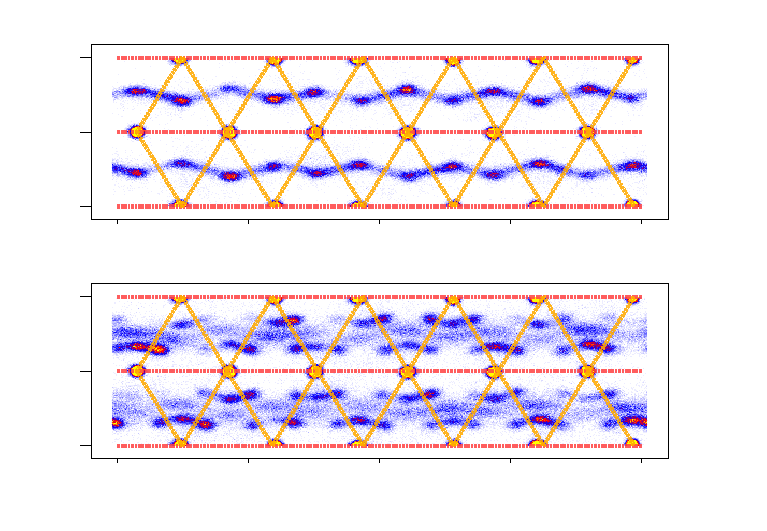
\includegraphics{imogolite-density-flat-small}}%
    \gplfronttext
  \end{picture}%
\endgroup

    \caption{Profils de densité sur les nanotubes "déroulés" pour l'oxygène de
    l'eau (haut), et l'hydrogène de l'eau (bas). La coordonnée circulaire
    correspond à une abscisse curviligne qui trace un cercle de rayon $R =
    \SI{6.5}{\AA}$ centré sur l'axe $z$. Sur tous les graphiques, les atomes
    d'oxygène internes apparaissent sous forme de points jaunes.}
    \label{fig:fr:imogolite:density:circular}
\end{figure}

Pour caractériser cette structure, nous avons calculé les profils de densité de
tous les types d'atomes, présenté en figure~\ref{fig:imogolite:density:xy} dans
le plan $xy$, comme si elles étaient vues du haut du nanotube (infini). En
regardant distribution de l'oxygène de l'eau \ce{O_w}, il est clair qu'il existe
deux populations différentes de molécules d'eau: de l'eau fortement structurée
adsorbée près de la surface interne et de l'eau plus désordonnée au centre du
nanotube. On observe également que les nanotubes sont légèrement déformés par
rapport à tube circulaire: les atomes de silicium sont placés dans une
disposition hexagonale. Cela est due à la symétrie de l'empilement des nanotubes
en faisceaux\cite{Amara2014}. Cette déformation est très faible, avec des
déplacements de Si de 0,1 à \SI{0,2}{\AA} tout au plus, les nanotubes
d'imogolite étant très rigides.

Une autre manière de visualiser l'adsorption est présentée en
figure~\ref{fig:fr:imogolite:density:circular}. Ici, la densité des atomes est
représentée par rapport à $z$ et une coordonnée circulaire, comme si une tranche
du nanotube avait été coupée et déroulée. On peut imaginer la surface interne
des nanotubes comme une séquence périodique de triangles, où chaque sommet est
un groupe silanol \ce{SiOH}. Sur la figure~\ref{fig:fr:imogolite:density:circular},
les lignes pointillées rouges indiquent les anneaux \ce{SiOH}, tandis que les
lignes pointillées orange indiquent ce maillage triangulaire. Ces triangles sont
isocèles avec deux angles de 66,5° et un angle de 47°. Au-dessus du centre de
chaque triangle se trouve un site potentiel d'adsorption d'eau. Cependant,
l'analyse des sites montre qu'aucun site voisin dans le même plan $xy$ ne peut
être occupé en même temps, étant donné qu'ils sont trop proches les uns des
autres. Au plus la moitié des sites d'adsorption seront donc occupés dans le
nanotube rempli d'eau. Nous pouvons aussi observer sur cette figure qu'il y a
une forte anisotropie du système. Là où les molécules d'eau peuvent se déplacer
dans un mouvement circulaire entre les sites dans le même plan $z$, il n'y a
aucune molécule passant d'un plan à l'autre. Il y a diffusion en surface des
molécules d'eau, mais seulement dans le plan $xy$. Ceci est corroboré par les
coefficients de diffusions, présentés en figure~\ref{fig:imogolite:msd}.

\begin{figure}[ht]
    \centering
    \raisebox{-0.5\height}{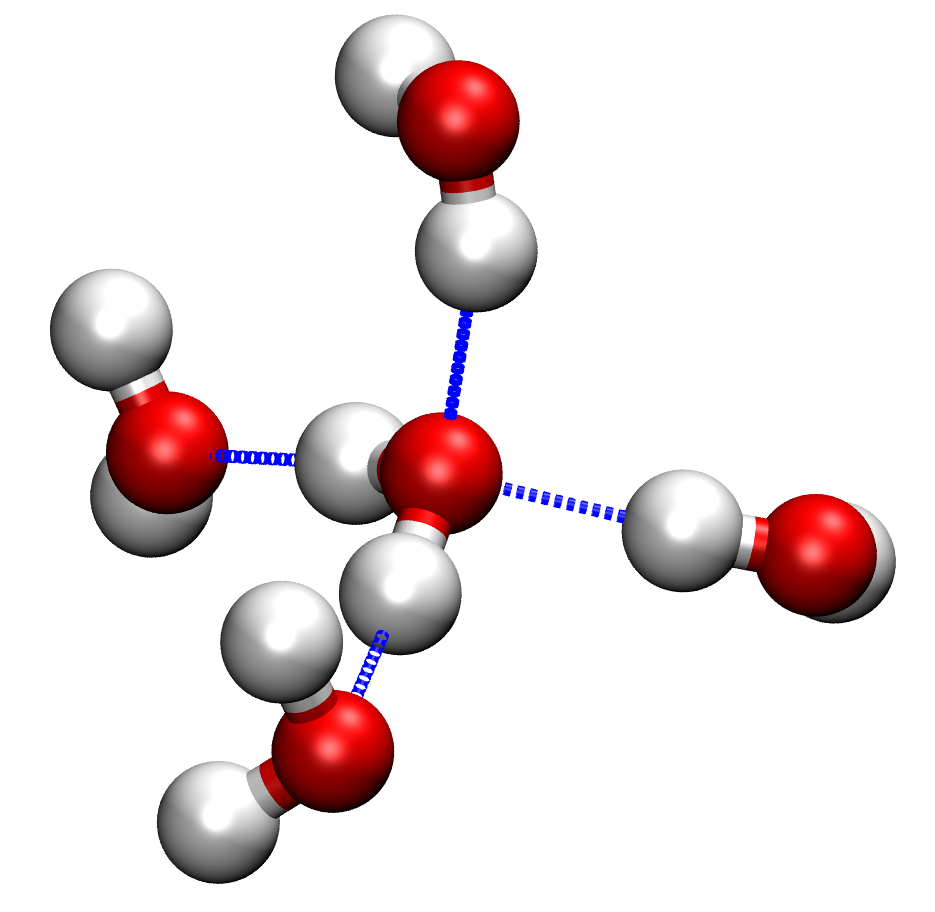
\includegraphics[width=0.2\textwidth]{figures/images/imogolite-hbonds-pattern-1}}
    \hskip2em
    \raisebox{-0.5\height}{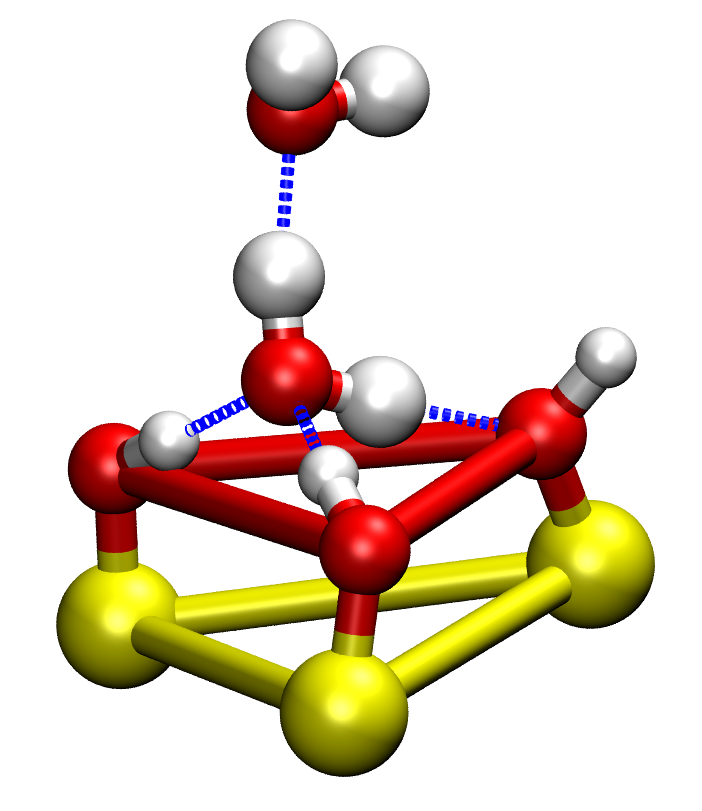
\includegraphics[width=0.2\textwidth]{figures/images/imogolite-hbonds-pattern-2}}
    \hskip2em
    \raisebox{-0.5\height}{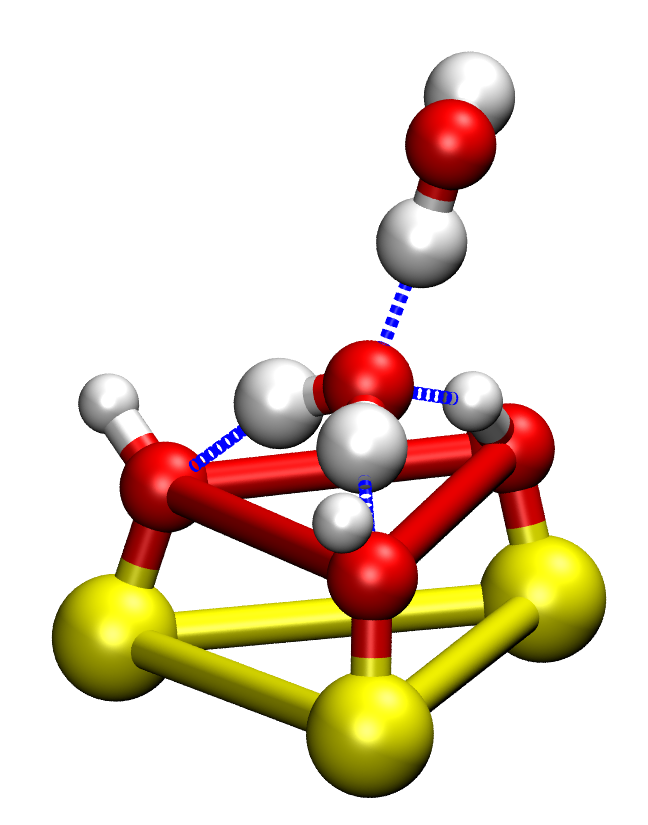
\includegraphics[width=0.2\textwidth]{figures/images/imogolite-hbonds-pattern-3}}
    \caption{Représentation des motifs de liaison hydrogène les plus courants
    pour l'eau dans un nanotube d'imogolite. De gauche à droite, ce sont les
    motifs 1, 2 et 3. Pour la numérotation des motifs, voir
    tableau~\ref{tab:imogolite:hbonds:patterns}.}
    \label{fig:fr:imogolite:hbonds:patterns}
\end{figure}

Afin de caractériser le réseau des liaisons hydrogène, nous avons classifié les
liaisons hydrogène en fonction du nombre de liaisons donnée et reçu avec d'autre
molécules d'eau et les silanols de surface. Les motifs les plus courants sont
représentés sur la figure~\ref{fig:fr:imogolite:hbonds:patterns}. Pour les
molécules adsorbées, le motif le plus courant est une molécule d'eau "verticale"
(motif 2). Un groupe hydroxyle de l'eau est orienté vers le centre du nanotube,
structurant l'eau adsorbée au-delà de la première couche. Le deuxième motif le
plus courant est une molécule d'eau située "à plat" sur la surface interne de
l'imogolite. Dans ce cas, la direction de la liaison hydrogène est moins
contrainte, ce qui explique la partie "diffuse" de la densité d'oxygène dans la
deuxième couche d'eau.

Nous avons montré que les interactions entre les molécules d'eau adsorbées sur
des sites voisins sont complexes, basées sur (1) l'exclusion d'un voisin le plus
proche, et (2) le nombre de liaisons hydrogène données (et acceptées) par les
molécules d'eau aux groupes silanol voisins. Maximiser le nombre de liaisons
hydrogène de ces règles crée de la frustration dans le système, ce qui conduit à
l'émergence d'un état fortement désordonné. Cette situation est très semblable
aux règles de Bernal-Fowler qui décrivent l'orientation des molécules d'eau dans
la glace\cite{Bernal1933}.

Enfin, nous avons également caractérisé la dynamique des molécules d'eau
confinées. Nous avons constaté qu'en plus de l'effet générique du ralentissement
de l'eau confinée, les fortes interactions des molécules d'eau avec les groupes
silanol donnent lieu à des constantes de temps comparables aux temps de séjour
typiques de l'eau dans les sites d'adsorption des protéines.

\clearpage
\section{Simulations hybride dans l'ensemble osmotique}

Le Monte-Carlo hybride est une amélioration de l'algorithme standard de
Monte-Carlo Metropolis qui permet de simuler plus efficacement des systèmes
complexes. Cette méthode est basée sur l'utilisation de courte simulations de
dynamique moléculaire pour générer une nouvelle conformation dans la chaîne de
Markov de la simulation Monte-Carlo. Pour pouvoir simuler l'adsorption dans des
matériaux poreux flexibles, il faut pouvoir échantillonner les mouvements
collectifs du matériau. Les techniques Monte-Carlo standard ne sont pas adapté à
cet effet, car elles doivent déplacer les atomes du système un par un pour être
efficaces. La dynamique moléculaire est capable de simuler les mouvements
collectifs, mais ne peut pas être utilisé pour des systèmes ouverts. Le
Monte-Carlo hybride permet d'améliorer l'efficacité de la simulation en
incorporant des informations sur la courbure locale de la surface d'énergie
potentielle.

J'ai implémenté la méthode Monte-Carlo hybride dans le logiciel de simulation
moléculaire Domino développé au sein du groupe. J'ai utilisé ce code pour une
étude préliminaire de l'adsorption du méthane \ce{CH4} dans un modèle
simplifié, sans charges, de la MOF-5 à \SI{300}{K}. Le calcul des interactions
électrostatiques n'était pas pris en charge par Domino. Bien que ce modèle ne
soit pas une représentation précise de la MOF-5, c'est un test intéressant pour
l'utilisation de simulations Monte-Carlo hybrides. L'isotherme prédite par cette
simulation est présentée en figure~\ref{fig:fr:hmc-mof5}

\begin{figure}[ht]
    \centering
    % GNUPLOT: LaTeX picture with Postscript
\begingroup
  \makeatletter
  \providecommand\color[2][]{%
    \GenericError{(gnuplot) \space\space\space\@spaces}{%
      Package color not loaded in conjunction with
      terminal option `colourtext'%
    }{See the gnuplot documentation for explanation.%
    }{Either use 'blacktext' in gnuplot or load the package
      color.sty in LaTeX.}%
    \renewcommand\color[2][]{}%
  }%
  \providecommand\includegraphics[2][]{%
    \GenericError{(gnuplot) \space\space\space\@spaces}{%
      Package graphicx or graphics not loaded%
    }{See the gnuplot documentation for explanation.%
    }{The gnuplot epslatex terminal needs graphicx.sty or graphics.sty.}%
    \renewcommand\includegraphics[2][]{}%
  }%
  \providecommand\rotatebox[2]{#2}%
  \@ifundefined{ifGPcolor}{%
    \newif\ifGPcolor
    \GPcolortrue
  }{}%
  \@ifundefined{ifGPblacktext}{%
    \newif\ifGPblacktext
    \GPblacktextfalse
  }{}%
  % define a \g@addto@macro without @ in the name:
  \let\gplgaddtomacro\g@addto@macro
  % define empty templates for all commands taking text:
  \gdef\gplbacktext{}%
  \gdef\gplfronttext{}%
  \makeatother
  \ifGPblacktext
    % no textcolor at all
    \def\colorrgb#1{}%
    \def\colorgray#1{}%
  \else
    % gray or color?
    \ifGPcolor
      \def\colorrgb#1{\color[rgb]{#1}}%
      \def\colorgray#1{\color[gray]{#1}}%
      \expandafter\def\csname LTw\endcsname{\color{white}}%
      \expandafter\def\csname LTb\endcsname{\color{black}}%
      \expandafter\def\csname LTa\endcsname{\color{black}}%
      \expandafter\def\csname LT0\endcsname{\color[rgb]{1,0,0}}%
      \expandafter\def\csname LT1\endcsname{\color[rgb]{0,1,0}}%
      \expandafter\def\csname LT2\endcsname{\color[rgb]{0,0,1}}%
      \expandafter\def\csname LT3\endcsname{\color[rgb]{1,0,1}}%
      \expandafter\def\csname LT4\endcsname{\color[rgb]{0,1,1}}%
      \expandafter\def\csname LT5\endcsname{\color[rgb]{1,1,0}}%
      \expandafter\def\csname LT6\endcsname{\color[rgb]{0,0,0}}%
      \expandafter\def\csname LT7\endcsname{\color[rgb]{1,0.3,0}}%
      \expandafter\def\csname LT8\endcsname{\color[rgb]{0.5,0.5,0.5}}%
    \else
      % gray
      \def\colorrgb#1{\color{black}}%
      \def\colorgray#1{\color[gray]{#1}}%
      \expandafter\def\csname LTw\endcsname{\color{white}}%
      \expandafter\def\csname LTb\endcsname{\color{black}}%
      \expandafter\def\csname LTa\endcsname{\color{black}}%
      \expandafter\def\csname LT0\endcsname{\color{black}}%
      \expandafter\def\csname LT1\endcsname{\color{black}}%
      \expandafter\def\csname LT2\endcsname{\color{black}}%
      \expandafter\def\csname LT3\endcsname{\color{black}}%
      \expandafter\def\csname LT4\endcsname{\color{black}}%
      \expandafter\def\csname LT5\endcsname{\color{black}}%
      \expandafter\def\csname LT6\endcsname{\color{black}}%
      \expandafter\def\csname LT7\endcsname{\color{black}}%
      \expandafter\def\csname LT8\endcsname{\color{black}}%
    \fi
  \fi
    \setlength{\unitlength}{0.0500bp}%
    \ifx\gptboxheight\undefined%
      \newlength{\gptboxheight}%
      \newlength{\gptboxwidth}%
      \newsavebox{\gptboxtext}%
    \fi%
    \setlength{\fboxrule}{0.5pt}%
    \setlength{\fboxsep}{1pt}%
\begin{picture}(7360.00,2820.00)%
    \gplgaddtomacro\gplbacktext{%
      \csname LTb\endcsname%%
      \put(543,595){\makebox(0,0)[r]{\strut{}$0$}}%
      \csname LTb\endcsname%%
      \put(543,886){\makebox(0,0)[r]{\strut{}$5$}}%
      \csname LTb\endcsname%%
      \put(543,1177){\makebox(0,0)[r]{\strut{}$10$}}%
      \csname LTb\endcsname%%
      \put(543,1468){\makebox(0,0)[r]{\strut{}$15$}}%
      \csname LTb\endcsname%%
      \put(543,1760){\makebox(0,0)[r]{\strut{}$20$}}%
      \csname LTb\endcsname%%
      \put(543,2051){\makebox(0,0)[r]{\strut{}$25$}}%
      \csname LTb\endcsname%%
      \put(543,2342){\makebox(0,0)[r]{\strut{}$30$}}%
      \csname LTb\endcsname%%
      \put(543,2633){\makebox(0,0)[r]{\strut{}$35$}}%
      \csname LTb\endcsname%%
      \put(645,409){\makebox(0,0){\strut{}$0$}}%
      \csname LTb\endcsname%%
      \put(1100,409){\makebox(0,0){\strut{}$10$}}%
      \csname LTb\endcsname%%
      \put(1554,409){\makebox(0,0){\strut{}$20$}}%
      \csname LTb\endcsname%%
      \put(2009,409){\makebox(0,0){\strut{}$30$}}%
      \csname LTb\endcsname%%
      \put(2464,409){\makebox(0,0){\strut{}$40$}}%
      \csname LTb\endcsname%%
      \put(2918,409){\makebox(0,0){\strut{}$50$}}%
      \csname LTb\endcsname%%
      \put(3373,409){\makebox(0,0){\strut{}$60$}}%
    }%
    \gplgaddtomacro\gplfronttext{%
      \csname LTb\endcsname%%
      \put(153,1614){\rotatebox{-270}{\makebox(0,0){\strut{}intake (\% wt)}}}%
      \csname LTb\endcsname%%
      \put(2009,130){\makebox(0,0){\strut{}pressure (bar)}}%
    }%
    \gplgaddtomacro\gplbacktext{%
      \csname LTb\endcsname%%
      \put(4427,595){\makebox(0,0)[r]{\strut{}$16.8$}}%
      \csname LTb\endcsname%%
      \put(4427,1003){\makebox(0,0)[r]{\strut{}$17$}}%
      \csname LTb\endcsname%%
      \put(4427,1410){\makebox(0,0)[r]{\strut{}$17.2$}}%
      \csname LTb\endcsname%%
      \put(4427,1818){\makebox(0,0)[r]{\strut{}$17.4$}}%
      \csname LTb\endcsname%%
      \put(4427,2225){\makebox(0,0)[r]{\strut{}$17.6$}}%
      \csname LTb\endcsname%%
      \put(4427,2633){\makebox(0,0)[r]{\strut{}$17.8$}}%
      \csname LTb\endcsname%%
      \put(4529,409){\makebox(0,0){\strut{}$0$}}%
      \csname LTb\endcsname%%
      \put(4950,409){\makebox(0,0){\strut{}$10$}}%
      \csname LTb\endcsname%%
      \put(5370,409){\makebox(0,0){\strut{}$20$}}%
      \csname LTb\endcsname%%
      \put(5791,409){\makebox(0,0){\strut{}$30$}}%
      \csname LTb\endcsname%%
      \put(6212,409){\makebox(0,0){\strut{}$40$}}%
      \csname LTb\endcsname%%
      \put(6632,409){\makebox(0,0){\strut{}$50$}}%
      \csname LTb\endcsname%%
      \put(7053,409){\makebox(0,0){\strut{}$60$}}%
    }%
    \gplgaddtomacro\gplfronttext{%
      \csname LTb\endcsname%%
      \put(3833,1614){\rotatebox{-270}{\makebox(0,0){\strut{}volume (\si{nm^3})}}}%
      \csname LTb\endcsname%%
      \put(5791,130){\makebox(0,0){\strut{}pressure (bar)}}%
    }%
    \gplbacktext
    \put(0,0){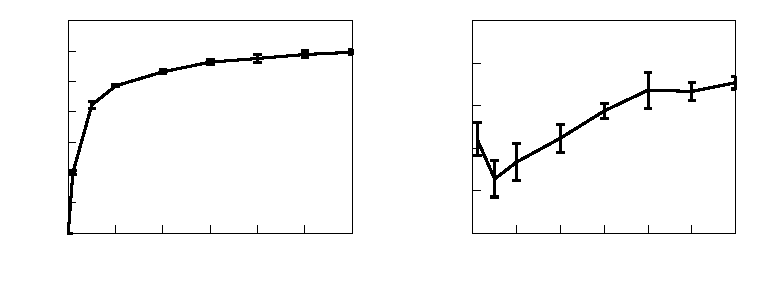
\includegraphics{hmc-mof5}}%
    \gplfronttext
  \end{picture}%
\endgroup

    \caption{Résultats de simulations Monte-Carlo hybride dans l'ensemble
    osmotique pour l'adsorption du méthane dans un modèle de MOF-5 simplifié.
    (gauche) isotherme d'adsorption à \SI{300}{K}, (droite) changement de volume
    pendant l'adsorption.}
    \label{fig:fr:hmc-mof5}
\end{figure}

Cette isotherme est de type I, comme prévu pour l'adsorption du méthane dans la
MOF-5. Contrairement aux simulations GCMC standard, cette isotherme intègre des
effets de flexibilité. Il est plus intéressant d'observer un comportement non
monotone dans les variations du volume en fonction de la pression. Nous
observons tout d'abord une faible contraction de la maille à basse pression,
avant l'expansion attendue à haute pression. Ce comportement de
contraction-expansion fait penser aux déformations induite par sorption dans
d'autres matériaux poreux\cite{Balzer2013, Mouhat2015}: la présence de quelques
molécules à l'intérieur des pores induit une contraction de tout le système. Une
autre façon de voir ce phénomène est d'imaginer les molécules à l'intérieur du
pore \emph{tirant} sur les parois. J'ai donc pu vérifier que la simulation
directe des déformations pendant l'adsorption était possible grâce aux méthodes
de Monte-Carlo hybride.

\clearpage
\section*{Conclusions}

Les travaux présentés dans cette thèse portent sur l'étude de l'adsorption et de
l'intrusion dans les matériaux flexibles nanoporeux, la déformation de ces
matériaux et le couplage entre les deux phénomènes. Le confinement d'un fluide à
l'intérieur d'un réseau poreux a des effets significatifs sur ses propriétés
thermodynamiques, du fait de la compétition entre les interactions avec les
interfaces et les interactions avec le fluide même. Cette compétition génère de
nouveaux comportements, tels que de nouvelles phases fluides et des transitions
entre ces phases, et est particulièrement présente dans les matériaux
nanoporeux, où la largeur typique du pore et la distance typique des
interactions sont du même ordre de grandeur. D'autre part, la présence d'un
fluide confiné peut également avoir des effets importants sur le solide
environnant, créant de nouvelles phases et modifiant l'équilibre entre plusieurs
phases méta-stables. C'est particulièrement poignant dans le cas des matériaux
nanoporeux flexibles, tels que de nombreux MOFs.

Comme ces matériaux sont relativement récents, leur flexibilité a souvent été
négligée et ce n'est que ces dernières années que la communauté scientifique a
commencé à en tenir compte. Un exemple d'un tel changement est présenté dans la
première section de ce résumé, avec l'incorporation de l'ensemble osmotique dans
la théorie de la solution adsorbée idéale (IAST) pour l'étude de la
co-adsorption des gaz, menant à la création de la théorie dite \emph{Osmotic
Framework Adsorbed Solution Theory} (OFAST). J'ai pu démontrer que la méthode
IAST est invalide \emph{par construction} pour le traitement de la co-adsorption
lorsque l'hôte adsorbant n'est pas inerte pendant l'adsorption. En particulier,
j'ai montré que IAST ne peut pas être utilisé pour la prédiction de la
co-adsorption de mélanges de fluides dans des matériaux présentant un
comportement d'ouverture de porte, et qu'il prédit une sélectivité non physique,
jusqu'à deux ordres de grandeur supérieurs à celle prédite par OFAST. Même
lorsque IAST n'est pas explicitement utilisé pour calculer la sélectivité dans
matériaux flexibles, il faut rester prudents en lorsque l'on compare des
isothermes de corps purs en présence de flexibilité. Les différences de pression
d'ouverture des isothermes peuvent conduire à des allégations de forte
sélectivité, lorsque l'on applique des concepts qui ne sont valables que pour
des matrices hôtes rigides.

Il faut aussi veiller à ne pas aller trop loin dans l'autre sens, et attribuer
tous les comportements observés à la flexibilité des matériaux. Dans la
quatrième section de ce résumé, j'ai utilisé des simulations de dynamique
moléculaire \abinitio pour expliquer l'origine d'une isotherme étagé pour
l'adsorption d'azote dans \ZIFCH3 et \ZIFCl, et son absence dans la structure
similaire \ZIFBr. J'ai montré que si le réseau se déforme pendant l'adsorption
pour \ZIFCH3 et \ZIFCl, les déformations ne changent pas le volume accessible et
la distribution des pores de ces matériaux. Au lieu de cela, l'augmentation de
l'absorption dans l'isotherme est liée à une réorganisation du fluide confiné
dans les pores, réorganisation qui ne se produit pas dans \ZIFBr en raison de la
différence de taille des pores. Il est donc fondamental de tenir compte à la
fois des effets de flexibilité et de confinement lors de l'étude de l'adsorption
dans les matériaux nanoporeux flexibles.

Il en va de même pour l'intrusion, cousin de l'adsorption. Dans les sections 4 et
5, j'ai utilisé des simulations moléculaires classiques pour étudier le
confinement sous haute pression de l'eau et de solutions d'électrolytes dans des
nanotubes d'imogolite et dans la \ZIF8. J'ai observé des effets de confinement
allant d'une organisation spatiale plus marquée, à des changements dans les
propriétés élastiques, et le ralentissement de la dynamique de l'eau. Il est
intéressant de noter que la présence d'ions à de forte concentrations peut avoir
les mêmes effets sur l'eau non confinée; structurant le réseau de liaisons
hydrogène et ralentissant la dynamique. L'intrusion de solution aqueuses dans un
matériau hydrophobe est un moyen prometteur de stocker et de dissiper l'énergie
mécanique. Il est possible d'ajuster le comportement et même de transformer un
système stockant de l'énergie à un système dissipatif d'énergie à la dissipation
en ajoutant des ions dans la solution aqueuse utilisée pour l'intrusion. J'ai
examiné l'impact des ions sur le comportement d'intrusion en utilisant des
simulations \emph{umbrella sampling} pour extraire le profil d'énergie libre
d'entrée dans la \ZIF8, montrant que les différents ions ont des barrières
différentes quand ils traversent les fenêtres de la \ZIF8. Cette étude est l'une
des premières sur le thème de l'intrusion d'électrolytes dans les MOF, et a
permis de mettre en lumière les comportements complexes qui émergent dans ces
systèmes.

La nécessité de tenir compte simultanément de l'adsorption et des déformations a
été un thème récurrent de toutes ces études. Mais les méthodes actuelles de
simulation ne permettent d'aborder qu'une seule dimension du problème: les
simulations de dynamique moléculaire peuvent décrire des déformations, mais la
modélisation de systèmes ouverts et donc l'adsorption n'est pas possible. Les
simulations de Monte-Carlo Metropolis peuvent être utilisées pour des systèmes
ouverts, mais elles ont du mal à échantillonner efficacement les déformations
collectives. Les simulations Monte-Carlo hybride sont une réponse possible à ce
dilemme, combinant l'efficacité de la dynamique moléculaire avec la polyvalence
des simulations Monte-Carlo (en particulier la possibilité d'échantillonner des
ensembles ouverts). La dernière section présente la méthode de simulation
Monte-Carlo hybride et son utilisation pour les simulations directes dans
l'ensemble osmotique.

Il y a une autre condition à remplir avant de pouvoir utiliser largement les
simulations d'ensembles osmotiques pour l'étude de l'adsorption et de
l'intrusion dans les cristaux nanoporeux flexibles: il nous faut pouvoir
calculer l'énergie liés à la flexibilité des matériaux et à leurs interactions
avec les fluides. Les méthodes \abinitio (comme la théorie de la fonctionnelle
de la densité) permettent de calculer avec précision l'énergie de systèmes
atomistiques arbitraires. Ces méthodes nécessitent malheureusement une grande
puissance de calcul, ce qui les empêche d'être utilisés en routine sur de grands
systèmes. Face à des systèmes d'une telle taille --- que ce soit en termes de
nombre d'atomes, d'échelle de temps des processus ou de criblage à haut débit
--- nous avons donc souvent recours aux champs de force classiques.

Les champs de force classiques sont soit \emph{précis}, c'est-à-dire qu'ils
reproduisent bien la surface d'énergie potentielle réelle, soit
\emph{transférables}, c'est-à-dire utilisables avec plusieurs systèmes
différents. Les champs de forces transférables actuels ne sont pas bien adaptés
pour décrire la flexibilité résultant des liaisons de coordination, il faut donc
créer de nouveaux champs de forces pour ces systèmes. Historiquement, la
paramétrisation de nouveaux champs de forces a été un processus assez long et
fastidieux. Depuis quelques années, de nouvelles techniques basées sur
l'apprentissage statistique ou \emph{Machine Learning} ont été mises au point
pour la dérivation constante et rapide de champs de force précis. Je présente
une de ces techniques dans la troisième section de ce résumé, que j'ai utilisée
pour obtenir des champs de force pour la \ZIF8 et certains de ses dérivés à
partir de données \abinitio. Ces techniques automatiques sont particulièrement
cruciales pour l'étude des MOFs en raison de la grande diversité de leurs
structures. J'espère que la disponibilité de champs de force précis et de
logiciels offrant des simulations de Monte-Carlo hybride facilitera
l'utilisation de simulations moléculaires pour concevoir de nouveaux matériaux
adaptés à des applications spécifiques.

\begin{center}
    \pgfornament[width=6cm,color=CTsemi]{88}
\end{center}

Ces travaux ouvrent des perspectives dans plusieurs directions. En ce qui
concerne les méthodes de simulation moléculaire, le Monte-Carlo hybride semble
être une technique puissante, utilisable avec une grande variété de systèmes.
Tout d'abord, la méthode Monte-Carlo hybride étant basée sur la théorie des
chaines de Markov et le critère de Metropolis convergera toujours vers la
distribution dans l'espace des phases de l'ensemble statistique voulu. Au
contraire, la dynamique moléculaire échantillonne par défaut l'ensemble
micro-canonique, et doit s'appuyer sur des thermostats et des barostats pour
échantillonner d'autres ensembles. Ces thermostats et surtout les barostats ne
sont pas tous égaux, et seuls certains algorithmes sont capables de générer
précisément l'ensemble souhaité. En même temps, les mouvements hybrides
améliorent grandement l'efficacité des simulations Monte-Carlo en tenant compte
de la courbure locale de la surface d'énergie potentielle.

Savoir s'il est possible de simuler des systèmes ouverts avec la dynamique
moléculaire reste aujourd'hui encore une question de recherche ouverte.
Inversement, de telles simulations sont couramment réalisées dans le cadre du
Monte-Carlo Grand Canonique. Le Monte-Carlo hybride pourrait ainsi être utilisé
pour la simulation d'ensembles ouverts et de systèmes dilués, tels que les
simulations à pH constant, la description de l'environnement ionique des
protéines ou la simulation de défauts dans les matériaux cristallins; améliorant
l'efficacité de ces simulations par rapport au Monte-Carlo classique et
permettant la simulation d'ensemble ouverts aux utilisateurs de dynamique
moléculaire. Grâce au critère d'acceptation de Metropolis, il n'est pas
nécessaire que la dynamique moléculaire courte utilisée par les mouvements
hybrides échantillonne un ensemble thermodynamique réel ou même un Hamiltonien
ayant un sens physique. Cette propriété pourrait être exploitée pour créer des
simulations Monte-Carlo encore plus efficaces, par exemple en insérant
progressivement de nouvelles molécules dans un système tout en relaxant son
environnement.

Une autre perspective concerne les champs de forces classiques et leur capacité
à reproduire avec précision les surfaces énergétiques potentielles. L'approche
traditionnelle lors de la création de champs de force a été de décomposer
l'énergie en une somme de termes dépendant de valeurs scalaires simples avec une
signification physique: distances, longueur de liaison, angles et angles
dièdres, \etc Ces valeurs scalaires sont ensuite combinées dans des
expressions mathématiques simples, par exemple des fonctions puissance ou
exponentielles. Dans cette approche la surface d'énergie potentielle ne peut pas
inclure d'effets à trois corps ou plus, ni reproduire avec précision la forme de
la surfaces d'énergie potentielle de référence. Les outils d'apprentissage
statistique, en particulier les réseaux neuronaux et les processus gaussiens,
peuvent apporter des améliorations à ces deux problèmes. Premièrement, la
capacité des réseaux de neurones à reproduire des fonctions arbitraires de
$\mathds{R}^n$ à $\mathds{R}$ peut réduire l'écart entre les surfaces d'énergie
potentielle de référence et du champ de force. Par exemple, au lieu d'imposer un
potentiel de Lennard-Jones, les réseaux neuronaux peuvent reproduire les
variations exactes de l'énergie. Deuxièmement, les algorithmes d'apprentissage
statistique peuvent être couplés à de meilleurs descripteurs de la structure
atomique, tenant compte des effets à plusieurs corps. Dans dernières années, de
multiples équipes scientifiques indépendantes ont travaillé à la conception,
l'entrainement et l'évaluation de ces champs de forces basé sur l'apprentissage
statistique et des descripteurs associés. À ma connaissance, ces méthodes n'ont
pas encore été utilisées pour l'étude de matériaux nanoporeux flexibles.

\vfill
\begin{center}
    \pgfornament[width=6cm,color=CTsemi]{75}
\end{center}
\vfill\vfill

\end{otherlanguage}

\OnlyInSubfile{\printglobalbibliography}

\end{document}
